% !TEX encoding = UTF-8 Unicode
\documentclass[a4paper]{article}
\usepackage[frenchb]{babel}
\usepackage{lmodern}
\usepackage{amssymb,amsmath}
\usepackage{ifxetex,ifluatex}
\usepackage{fixltx2e} % provides \textsubscript
\ifnum 0\ifxetex 1\fi\ifluatex 1\fi=0 % if pdftex
  \usepackage[T1]{fontenc}
  \usepackage[utf8]{inputenc}
\else % if luatex or xelatex
  \ifxetex
    \usepackage{mathspec}
  \else
    \usepackage{fontspec}
  \fi
  \defaultfontfeatures{Ligatures=TeX,Scale=MatchLowercase}
\fi
% use upquote if available, for straight quotes in verbatim environments
\IfFileExists{upquote.sty}{\usepackage{upquote}}{}
% use microtype if available
\IfFileExists{microtype.sty}{%
\usepackage{microtype}
\UseMicrotypeSet[protrusion]{basicmath} % disable protrusion for tt fonts
}{}
\usepackage{hyperref}
\PassOptionsToPackage{usenames,dvipsnames}{color} % color is loaded by hyperref
\hypersetup{unicode=true,
            pdftitle={Une description taxonomique du genre Cecropia (Urticaceae): Réalisation d'une clef d'identification multi-entrées},
            pdfauthor={Nguyen Le Xuan bach},
            colorlinks=true,
            linkcolor=blue,
            citecolor=blue,
            urlcolor=blue,
            breaklinks=true}

\urlstyle{same}  % don't use monospace font for urls
\usepackage{natbib}
\bibliographystyle{apalike}
\usepackage{longtable,booktabs}
\IfFileExists{parskip.sty}{%
\usepackage{parskip}
}{% else
\setlength{\parindent}{0pt}
\setlength{\parskip}{6pt plus 2pt minus 1pt}
}
\setlength{\emergencystretch}{3em}  % prevent overfull lines
\providecommand{\tightlist}{%
  \setlength{\itemsep}{0pt}\setlength{\parskip}{0pt}}
\setcounter{secnumdepth}{5}
% Redefines (sub)paragraphs to behave more like sections
\ifx\paragraph\undefined\else
\let\oldparagraph\paragraph
\renewcommand{\paragraph}[1]{\oldparagraph{#1}\mbox{}}
\fi
\ifx\subparagraph\undefined\else
\let\oldsubparagraph\subparagraph
\renewcommand{\subparagraph}[1]{\oldsubparagraph{#1}\mbox{}}
\fi

%%% Use protect on footnotes to avoid problems with footnotes in titles
\let\rmarkdownfootnote\footnote%
\def\footnote{\protect\rmarkdownfootnote}


  \title{Une description taxonomique du genre Cecropia (Urticaceae): Réalisation
d'une clef d'identification multi-entrées}
    \author{Nguyen Le Xuan bach}
      \date{Février -- Juin 2012}
\newpage
\usepackage{booktabs}
\usepackage{amsthm}
\usepackage{lipsum} % Dummy text.
\makeatletter
\def\thm@space@setup{%
  \thm@preskip=8pt plus 2pt minus 4pt
  \thm@postskip=\thm@preskip
}
\makeatother
\usepackage{pdfpages}
\usepackage[left=2.5cm,right=2.5cm,top=2.5cm,bottom=2.5cm]{geometry}
%=====================
%change font size
\usepackage{scrextend}
\changefontsizes{13pt}
%=====================

%++++++++++++++++
%THUT DAU DONG
%\parindent 0ex %khong thut dau dong
\setlength{\parindent}{1cm}%thụt đầu dòng 1 cm
%\setlength{\parskip}{1em} %khoang cach giua 2 doan van
%\renewcommand{\baselinestretch}{1.25} %khoảng cách giua 2 dòng
\linespread{1.5} %khoảng cách giua 2 dòng
%++++++++++++++++
\usepackage{fontspec}
\usepackage{float}
\usepackage{setspace}
\usepackage{caption}
\captionsetup[table]{font={stretch=1}}     %% change 1.2 as you like
\captionsetup[figure]{font={stretch=1}}    %% change 1.2 as you like
 %% or
 %% \captionsetup{font={stretch=1.2}}  %% this affects both figure and table
\usepackage{longtable}
\usepackage{tabularx}
\usepackage[nottoc, notlot, notlof]{tocbibind}

\usepackage{amsthm}
\newtheorem{theorem}{Theorem}[section]
\newtheorem{lemma}{Lemma}[section]
\theoremstyle{definition}
\newtheorem{definition}{Definition}[section]
\newtheorem{corollary}{Corollary}[section]
\newtheorem{proposition}{Proposition}[section]
\theoremstyle{definition}
\newtheorem{example}{Example}[section]
\theoremstyle{definition}
\newtheorem{exercise}{Exercise}[section]
\theoremstyle{remark}
\newtheorem*{remark}{Remark}
\newtheorem*{solution}{Solution}
\begin{document}
\pagenumbering{gobble}
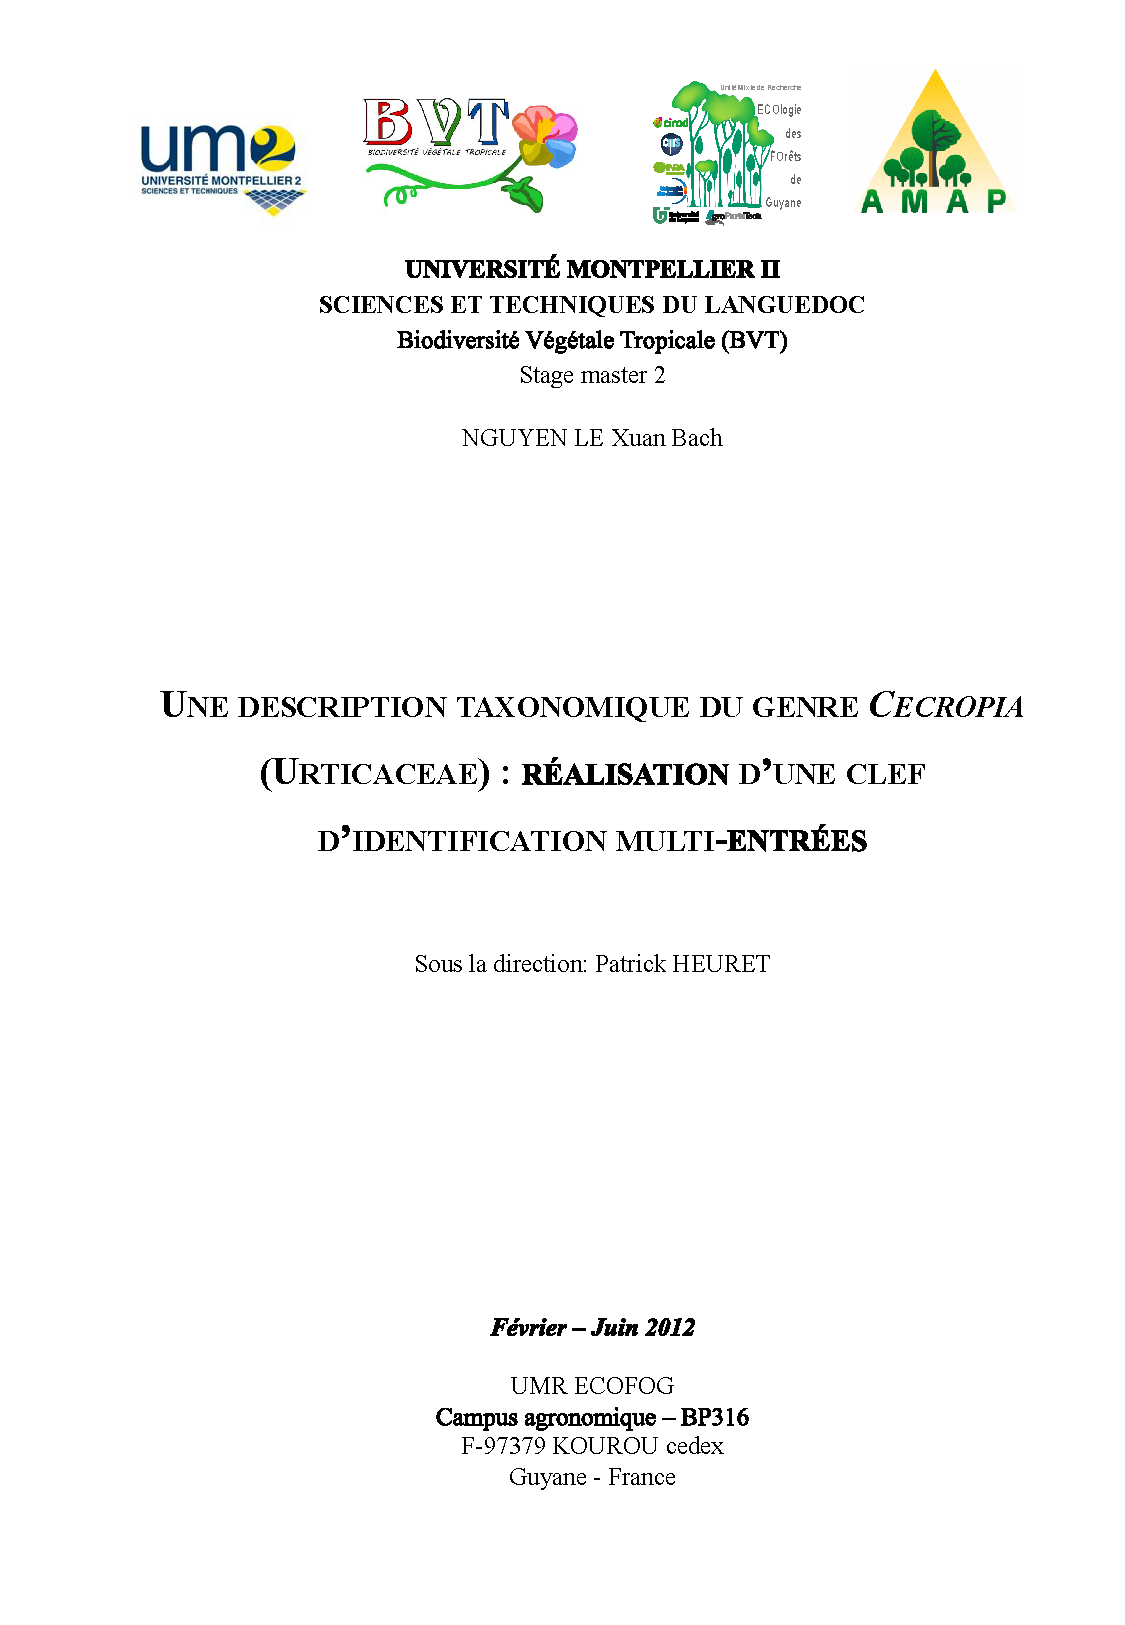
\includepdf[pages={-}, scale=1]{cover.pdf}
\maketitle



{
\hypersetup{linkcolor=black}
\setcounter{tocdepth}{2}
\newpage
\tableofcontents
}
\newpage
\pagenumbering{roman}

\section*{Résumé et Abstract}\label{resume-et-abstract}
\addcontentsline{toc}{section}{Résumé et Abstract}

\textbf{Résumé}

\emph{Cecropia} Loefl. (Urticaceae) est un des genres les plus
emblématique des néotropiques. Il regroupe des espèces d'arbres
pionniers avec une importance écologique toute particulière puisqu'ils
constituent les peuplements initiaux de la succession forestière et des
peuplements de forêts secondarisées. Bien que plusieurs espèces de
\emph{Cecropia} soient étudiées dans des domaines très divers, la
systématique du genre est paradoxalement très mal connue et la
détermination des espèces reste difficile malgré la publication d'un
volume de Flora Neotropica par Berg et Franco-Rosselli (2005). Dans ce
travail, je propose une nouvelle lecture de cet ouvrage en construisant
une clef de détermination multi-entrées et illustrée, pour les 61
espèces du genre, à l'aide de la plate-forme Xper2. J'associe à ce
travail une base de donnée photographique ainsi que des fiches de
reconnaissance illustrées pour 22 espèces. Afin de stimuler la collecte
de nouvelles informations sur ce genre dans un esprit de « science
citoyenne », je propose un protocole de prise de vue photographique,
facilement réalisable par le néophyte, et permettant d'accéder aux
caractères clefs pour l'identification des espèces et la compréhension
de leur variabilité phénotypique.

\textbf{Mots clés}: \emph{cecropia; protocole; XPER; logiciel
d'identification}.

\textbf{Abstract} \emph{Cecropia} Loefl. (Urticaceae) is one of the most
important genus of the neotropics. It includes several species of
pioneer trees. They play an important role in the initial stands of
forest succession and stands of secondary forest. Several species of
\emph{Cecropia} are studied in different fields of research; however,
systematics of the genus is paradoxically poorly known. Species
identification remains difficult despite the availability of dichotomous
key and description in a volume of Flora Neotropica that edited by Berg
and Franco-Rosselli (2005). In the present study, I propose a new
interpretation of this publication by a multi-entry key developed with
the Xper2 platform to identify 61 Cecropia species. Furthermore, I
constructed a photographic library and edited rapid color guides for 22
species. To motivate new observations and ``citizen science''
opportunity, I suggested a protocol to take pictures that is easily to
follow by the novice; and to access to key characters for the
identification of species and understanding of their phenotypic
variability.

\textbf{Key words}: \emph{cecropia; protocol; XPER; identification
software} \pagebreak

\pagenumbering{arabic}

\section{Introduction}\label{intro}

Ce travail s'est déroulé du 15/02/2012 au 15/06/2012 à l'Unité Mixte de
Recherche « Ecologie des forêts de Guyane » (ECOFOG) en Guyane française
qui dépend de 5 tutelles : AgroParisTech (745), l'INRA (745), le CNRS
(8172), le CIRAD (93) et l'Université Antilles-Guyane (43). ECOFOG fait
partie du laboratoire d'excellence « Centre d'Etude de la Biodiversité
Amazonienne (Labex CEBA) » qui réunit un ensemble d'acteurs de la
recherche et de l'enseignement supérieur en Guyane, aux Antilles et en
métropole, autour d'un contenu scientifique d'excellence sur le thème de
la biodiversité amazonienne : environnement, écologie, biodiversité,
santé et écotechnologie. Ce travail a bénéficié d'une aide de l'Etat
gérée par l'Agence Nationale de la Recherche au titre du programme
Investissements d'avenir portant la référence ANR-10-LABX-0025

\emph{Cecropia} Loefl. est un des genres les plus emblématique des
néotropiques \citep{Berg2005}. Il regroupe des espèces d'arbres
pionniers qui colonisent les chablis forestiers ainsi que les zones
déboisées et défrichées pleinement exposées à la lumière. \emph{Cecropia
spp.} se distribuent naturellement du sud du Mexique jusqu'au nord de
l'Argentine ainsi qu'aux Antilles (Fig. \ref{fig:fig1}). Ce sont des
arbres de dimensions souvent restreintes (5-15 m) bien que certaines
espèces puissent culminer à une quarantaine de mètres (\emph{e.g.~C.
sciadophylla}). Ce sont des plantes dioïques conformes au modèle
architectural de Rauh \citep{HalleOledeman1970, Halle1978}. L'ensemble
des axes est orthotrope ; le tronc porte des étages de branches bien
marqués (ramification rythmique), et développe souvent à sa base des
racines échasses qui donnent à l'arbre une silhouette caractéristique.
La floraison est latérale. Les axes, peu nombreux, sont formés d'une
succession de nœuds facilement repérables tout au long de la vie de la
plante à cause de la cicatrice circulaire laissée par le capuchon
stipulaire, \emph{i.e.} la calyptre \citep{Heuret2002, Zalamea2008}. Les
feuilles sont simples, plus ou moins lobées, de grande taille et sont
disposées autour de l'axe selon une phyllotaxie alterne spiralée.





\begin{figure}[H]

{\centering 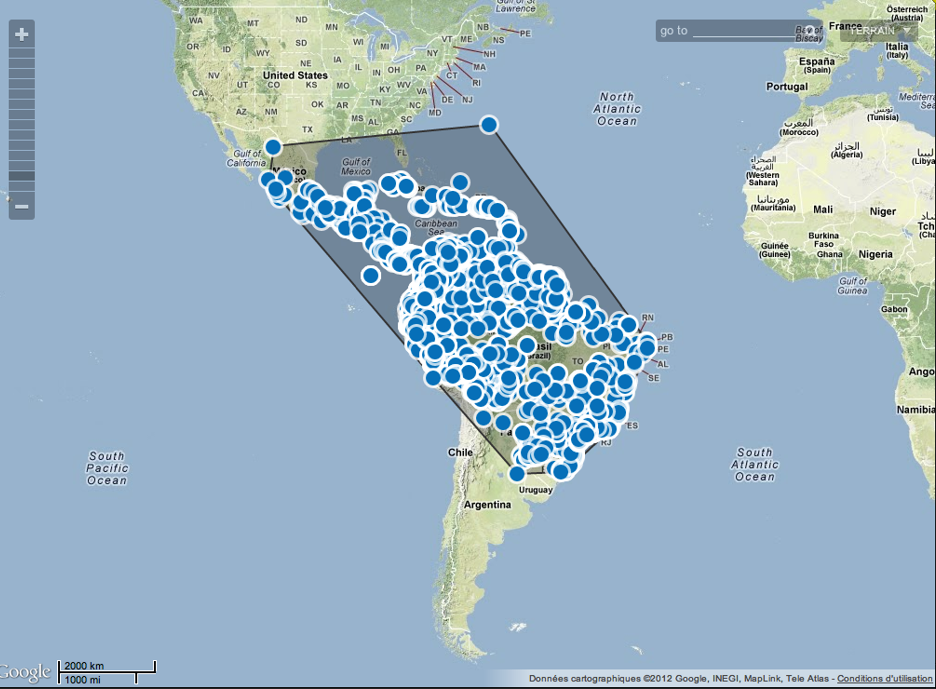
\includegraphics[width=0.8\linewidth]{figure/fig1} 

}

\caption{Carte de repartition du genre \emph{Cecropia} (Source data
GPS Zalamea et al. \citeyearpar{Zalamea2011} avec Google Map© dans
\url{http://geocat.kew.org})}\label{fig:fig1}
\end{figure}






\begin{figure}[H]

{\centering 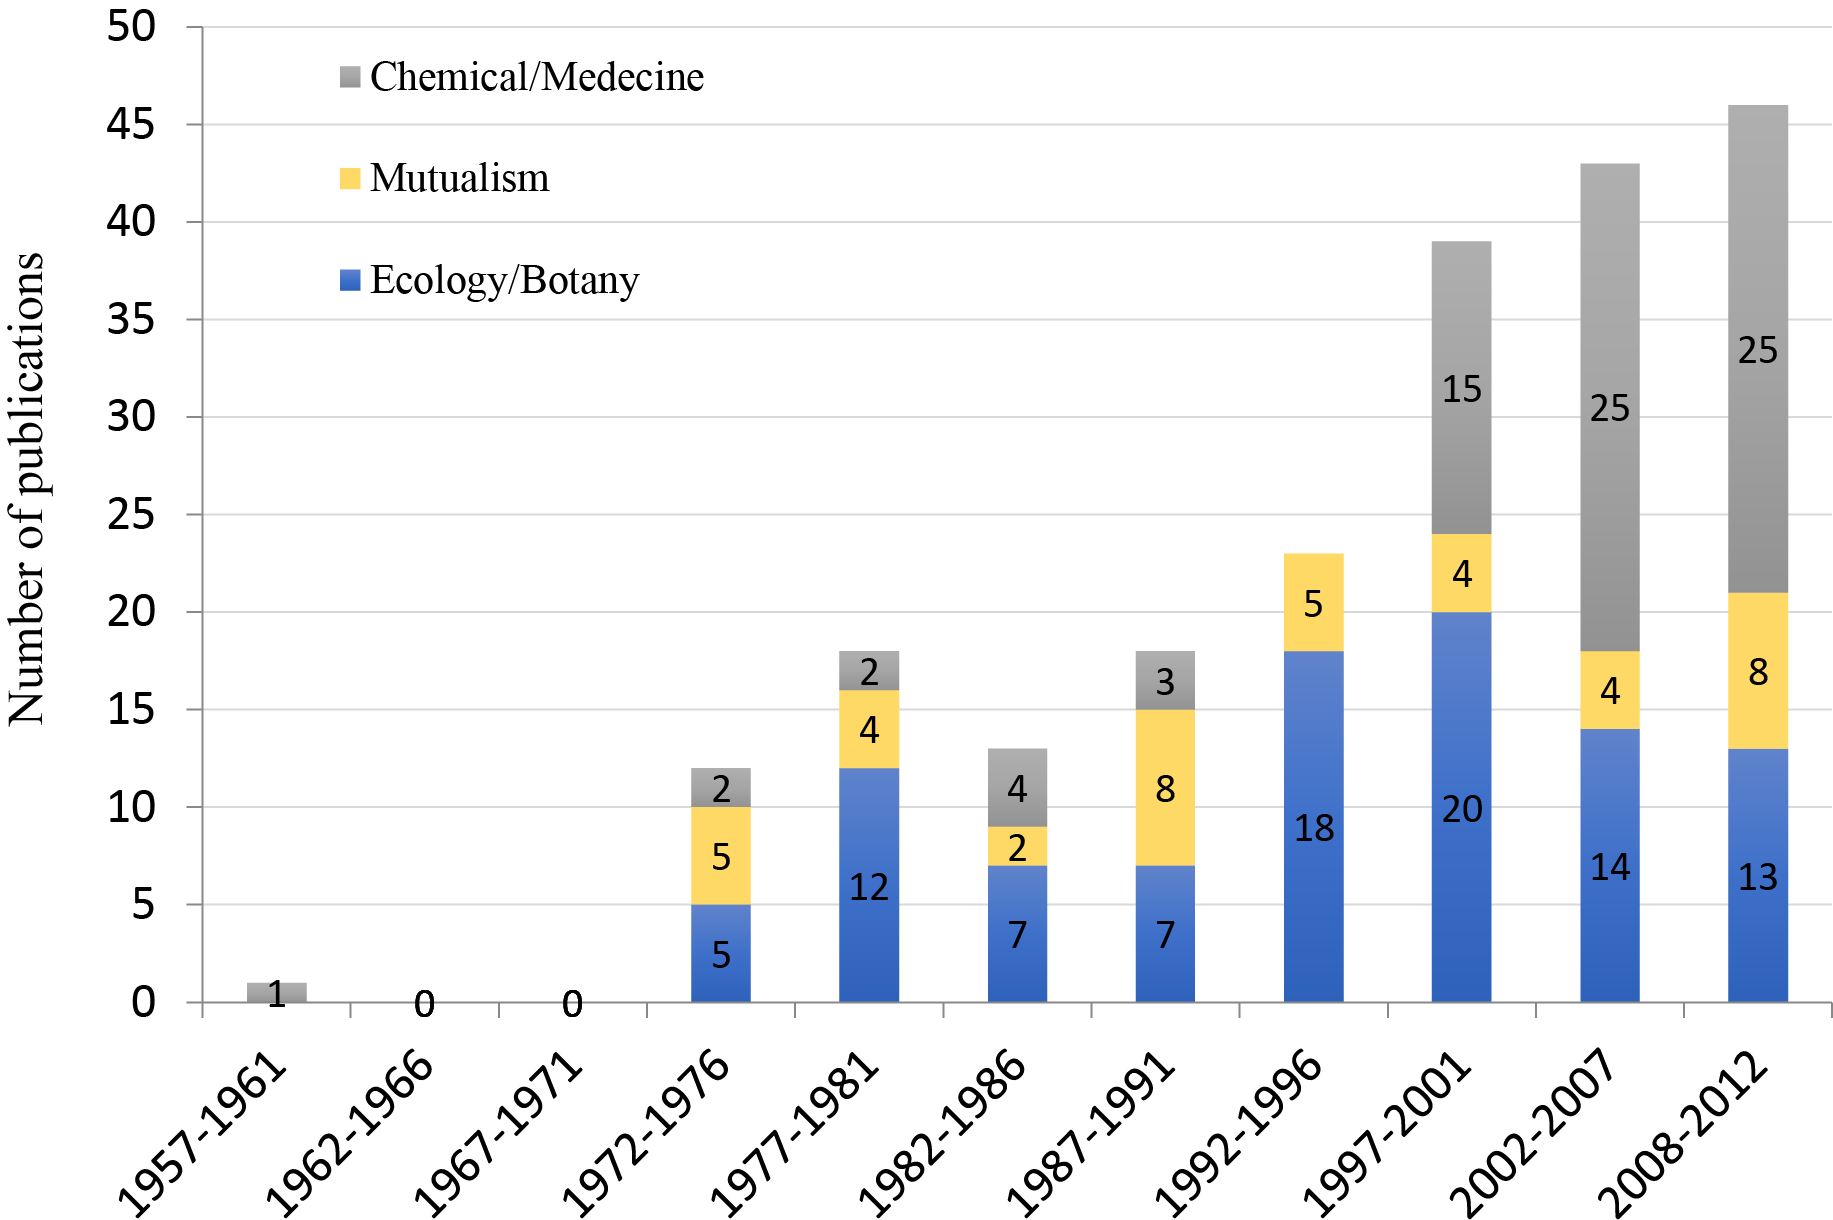
\includegraphics[width=1\linewidth]{figure/fig2} 

}

\caption{Nombre de publications concernant le genre \emph{Cecropia}
selon trois grands thèmes et par tranche de cinq années. (Source : Web
of Science / comptabilisé si le titre de l'article contient
`\emph{Cecropia}')}\label{fig:fig2}
\end{figure}

Les \emph{Cecropia} sont intéressants à plus d'un égard:

\begin{enumerate}
\def\labelenumi{(\roman{enumi})}
\item
  Leur caractéristique d'arbres pionniers leur confère une importance
  écologique toute particulière puisqu'ils constituent les peuplements
  initiaux de la succession forestière et des peuplements de forêts
  secondarisées. A ce titre, \emph{C. obtusa} et \emph{C. sciadophylla}
  se sont révélées être d'excellentes plantes marqueurs permettant de
  dater très exactement l'âge d'une perturbation. En effet, ces deux
  espèces montrent une ramification et une floraison annuelle laissant
  des cicatrices caractéristiques tout au long de la vie de la plante et
  mettent en place un nombre de feuille par an d'une extraordinaire
  régularité permettant de dater aisément l'âge d'un individu et donc de
  la perturbation à l'origine de son installation
  \citep{Davis1970, Heuret2002, Zalamea2008, Zalamea2009} . Une bonne
  connaissance de leur écologie est donc capitale pour comprendre les
  mécanismes de résilience/cicatrisation des forêts perturbées;
\item
  introduit à plusieurs reprises dans des jardins botaniques en dehors
  de leurs aires de distributions, plusieurs espèces se sont échappées
  et sont considérées aujourd'hui comme envahissantes. Par exemple,
  \emph{C. peltata} est présent en Afrique de l'Ouest (Cameroun) où il
  concurrence son homologue africain \emph{Musanga cecropioides}
  \citep{McKey1988}. \emph{C. peltata} et \emph{C. schreberiana} se
  trouvent sur la liste de l'UICN des 100 espèces exotiques
  envahissantes parmi les plus néfaste au monde
  \href{http://www.issg.org/database/welcome/}{(link)}. Les
  introductions de \emph{Cecropia} sont cependant souvent mal
  identifiées et il existe peu de connaissances sur l'état d'invasion et
  la dynamique de colonisation des \emph{Cecropia} dans leur nouvel
  environnement \citep{Webber2011};
\item
  vivant tous en association avec des fourmis (en majorité le genre
  \emph{Azteca}), les \emph{Cecropia} sont de parfaits sujets pour les
  travaux visant à comprendre la relation de mutualisme entretenue entre
  plantes et insectes
  \citep{Janzen1973, Folgarait1994, Gianoli2008, Dejean2009};
\item
  de par leur architecture simple, et l'expression de processus de
  croissance cycliques (e.g.~ramification rythmique), ils constituent
  d'excellents arbres `modèles' pour définir et évaluer des modèles
  mathématiques de type structure-fonction pour comprendre et simuler le
  architectural des arbre \citep{Letort2012};
\item
  enfin, les \emph{Cecropia} sont traditionnellement utilisés par les
  populations locales dans la composition de différents remèdes : la
  sève est utilisée contre les verrues, les cals, les ulcères, et les
  diarrhées ; les feuilles sont utilisées contre les troubles
  cardiaques, le traitement de l'asthme, et comme diurétique
  \citep{Berg2005}. Plusieurs propriétés anti-inflammatoires et
  antidiabétiques ont ainsi été mises en évidence \citep{Costa2011}. En
  fait, depuis une dizaine d'années, la moitié des travaux publiés sur
  les \emph{Cecropia} concernent à présent les propriétés
  chimique/pharmaceutique de certaines espèces (Fig. \ref{fig:fig2}).
  Certains médicaments homéopathiques sur le marché contiennent déjà des
  extraits de \emph{C. palmata} (Poconeol N°20, N°48)
  \href{http://www.vidal.fr/Substance/cecropia_palmata-843.htm}{(link)}.
\end{enumerate}

Bien que plusieurs espèces de \emph{Cecropia} soient étudiées pour des
aspects très divers, la systématique du genre est paradoxalement très
mal connue. D'un point de vue taxonomique, le genre \emph{Cecropia}
appartenait à la famille des Cecropiaceae, qui a été recombinée
récemment en tribu des Cecropieae dans les Urticacées par l'APG III
\citep{apg3}. Les Cecropieae comptent six genres : trois néotropicaux
(\emph{Cecropia, Pourouma, Coussapoua}), deux africains (\emph{Musanga,
Myrianthus}) et un asiatique (\emph{Poikilospermum}). Le genre
\emph{Cecropia} a fait l'objet d'une révision récente au travers d'un
volume de la collection Flora Neotropica \citep{Berg2005}\footnote{Faisant
  référence à cet ouvrage tout au long de ce document, je simplifierai
  sa citation par B\&FR2005} et 61 espèces, et deux sous-espèces, sont
reconnues. Malgré ce travail remarquable, plusieurs points méritent
d'être soulignés :

\begin{enumerate}
\def\labelenumi{(\roman{enumi})}
\item
  Il n'existe à ce jour aucune phylogénie du genre\footnote{A notre
    connaissance, un projet est actuellement en cours et mené par G.
    Weiblen (Université du Minnesota) et S. Madrinan (Universidad de Los
    Andes, Colombie) sur quelques espèces de Colombie. Un poster a été
    présenté à la conférence
    \href{http://2009.botanyconference.org/engine/search/index.php?func=detail\&aid=56}{(Botany2009)}}
  et les espèces ne sont identifiées qu'au travers d'une approche
  taxonomique traditionnelle. B\&FR2005 en soulignent bien les limites
  en introduction de leur ouvrage (p.7). Tout d'abord, il n'existe que
  très peu de collections d'herbiers. Dans une étude portant sur la
  phénologie du genre au travers de l'observation de spécimens
  d'herbiers \citep{Zalamea2011} ont pu observer dans les principaux
  herbiers mondiaux 3668 spécimens fertiles pour l'ensemble des 61
  espèces. Certaines espèces ne sont décrites qu'au travers de très peu
  d'échantillons (\emph{e.g.~C. silvae} : 5 échantillons ; Fig.
  \ref{fig:fig3}). Les collecteurs rechignent en effet à collecter ce
  qui semble être une banalité (au premiers abords, tous les
  \emph{Cecropia} se ressemblent), avec des feuilles de grandes
  dimensions difficiles de mettre en herbiers et la présence de fourmis
  agressives qui jouent leur rôle dissuasif. Par ailleurs, la dioécie
  ajoute une difficulté supplémentaire puisque les deux sexes ne sont
  pas systématiquement récoltés. Ainsi, beaucoup d'espèces restent
  méconnues comme en témoigne la figure 6-2 issue de la thèse de
  \citet{Zalamea2009} qui présente pour chaque espèce (i) le nombre
  d'échantillons d'herbiers récoltés et consultable dans les grand
  herbiers internationaux, (ii) le nombre total de citation google © ou
  (iii) le nombre de citation Web of science ou l'espèce figure dans le
  titre ou les mots-clefs d'un article. En l'état actuel des choses,
  nous avons donc très peu d'éléments pour statuer sur la distribution
  géographiques des espèces, leur variations morphologiques et les
  causes de cette variabilité (étude de la plasticité) et leur existence
  réelle alors que des phénomènes d'hybridation sont fortement suspectés
  \citep{Webber2011};
\item
  Le travail de B\&FR2005 propose une clef dont l'entrée principale
  repose sur la localisation géographique. Ces auteurs argumentent leur
  choix en disant qu'une clef générale aurait des entrées trop faibles
  en raison de la dioécie et de la grande variabilité des caractères.
  Or, comme nous l'avons vu, de nombreuses espèces de \emph{Cecropia} se
  trouvent aujourd'hui en dehors de leur aire d'origine et sont alors
  envahissantes. Les problèmes d'identification sont courants et donnent
  lieu à de vives polémiques \citep{Sheil2011a, Sheil2011b, Webber2011};
\item
  Les critères décrits par B\&FR2005 sont ont été essentiellement
  observés sur planches d'herbiers et certains se révèlent difficilement
  utilisables sur le terrain. Les critères tels que les couleurs ou
  certaines dimensions (diamètre de pétiole ou de l'axe des
  inflorescences) sont particulièrement sensibles à la déshydratation
  subie pour le conditionnement en herbiers;
\item
  Seules 34 sur 61 espèces sont illustrées aux travers de planches de
  dessin. Par ailleurs beaucoup de critères utilisés pour la
  discrimination des espèces ne sont pas illustrés ce qui rend leur
  identification difficile pour le néophyte;
\item
  Le dernier problème est inhérent aux clefs dichotomiques : la non
  indentification d'un seul caractère bloque la poursuite de
  l'identification.
\end{enumerate}

Ainsi, bien que ce volume de \emph{Flora Neotropica} soit sans conteste
une avancée majeure et une synthèse remarquable pour l'identification
des différentes espèces, l'exercice reste souvent compliqué sur le
terrain. Compte de tenue de l'importance du genre dans les différents
domaines cités, une bonne identification taxonomique est un pré-requis
absolument indispensable à ces études. Comme le souligne
\citep{Evans2007} à propos plantes introduites invasives,
l'identification correcte d'une espèce et une compréhension solide de sa
biologie constitue l'exigence minimale pour la lutte biologique ciblée.

Quelles voies pouvons-nous suivre pour progresser dans la compréhension
de la systématique du genre \emph{Cecropia} et l'identification des
espèces ? La motivation de nouvelles collectes et observations au
travers d'une approche collaborative en réseau est absolument nécessaire
pour aborder un genre avec une aire de répartition aussi vaste. Un tel
réseau ne peut exister que si des protocoles et des outils communs sont
partagés afin d'assurer une homogénéité des données récoltées. Dans ce
contexte les objectifs de ce travail ont été de (i) construire une clef
de détermination multi-entrées et illustrée pour le genre
\emph{Cecropia} à l'aide du logiciel Xper2
\href{http://lis-upmc.snv.jussieu.fr/lis/?q=ressources/logiciels/xper2}{(link)}
en se basant dans un premier temps sur le travail de B\&FR2005 ; (ii) de
regrouper des illustrations photographiques pour l'ensemble des espèces
(planches d'herbiers et plantes fraiches), (iii) de tester cette clef
sur les différents Cecropia trouvés en Guyane Française et (iv) de
proposer des protocoles de description et de prise de vue photographique
des specimens et mener une réflexion sur les modalités de mise en place
d'un réseau d'observation international de ce genre.







\begin{figure}[H]

{\centering 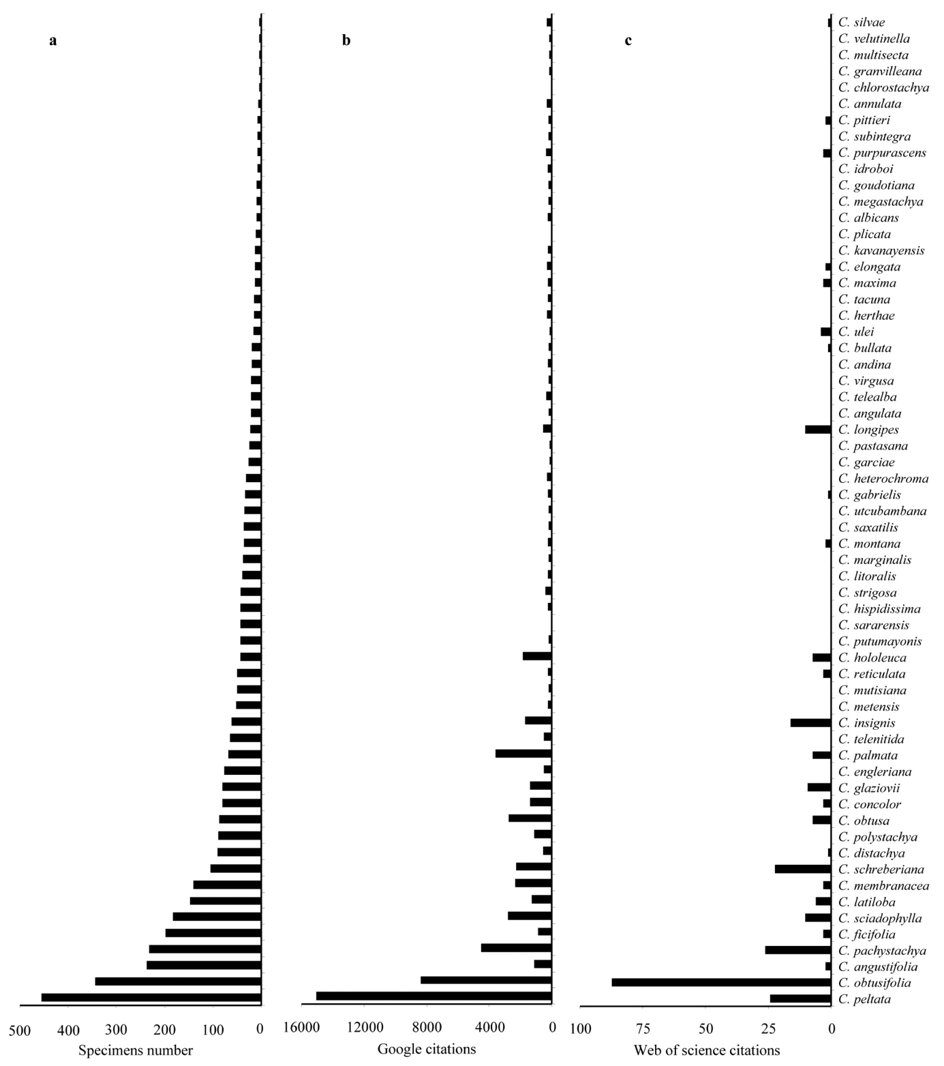
\includegraphics[width=1\linewidth]{figure/fig3} 

}

\caption{Pour chaque espèce de \emph{Cecropia} : (a) le nombre
d'échantillons d'herbiers disponibles, (b) le nombre total de citation
Google © et (c) le nombre de citation Web of science ou l'espèce figure
dans le titre ou les mots-clefs d'un article. Source: P.C Zalamea
\citeyearpar{Zalamea2009}}\label{fig:fig3}
\end{figure}

\pagebreak

\section{Matériels et Méthodes}\label{materiels-et-methodes}

\subsection{Construction d'une base de donnée
photographique}\label{construction-dune-base-de-donnee-photographique}

Une première étape de ce travail a été de regrouper le plus possible
d'illustrations disponibles sur \emph{Cecropia} et de les assembler dans
une base de donnée sous le logiciel Aperture©
\href{http://www.apple.com/fr/aperture/}{(link)}. Pour les plantes
fraiches, j'ai intégré les photographies des photothèques personnelles
de différents botanistes (P. Heuret, P.C. Zalamea, D. Sabatier, M.
Kostlin, J. Grosfeld, E. Nicolini) et j'ai moi-même photographié de
nombreux spécimens en Guyane Française. J'y ai également intégré
plusieurs photographies disponibles sur internet sous une licence «
Creative Commons
\href{http://fr.wikipedia.org/wiki/Creative_Commons}{(link)}» comme
celles publiées par le Field Museum de Chicago
\href{http://fm2.fieldmuseum.org/plantguides/results.asp?genus=Cecropia}{(link)}.
J'ai bénéficié également de photographies de planches d'herbiers prises
par P.C. Zalamea dans les herbiers de New-York (NY) et du muséum
national de Paris (P). J'ai complété cela avec de nombreuses
photographies téléchargées depuis les sites internet des principaux
herbiers internationaux
\href{http://en.wikipedia.org/wiki/Virtual_herbarium}{(link)} (Kew
\href{http://apps.kew.org/herbcat/navigator.do}{(link)}, Field Museum
\href{http://fm1.fieldmuseum.org/vrrc/}{(link)}, Missouri Botanical
Gardens \href{http://www.tropicos.org/ImageSearch.aspx}{(link)} ou bien
sous Jstor \href{http://plants.jstor.org/}{(link)}. Enfin, à l'aide d'un
microscope digital KEYENCE VHX-500F, j'ai également pris plusieurs
clichés de détails (e.g.~types de poils, grain de pollen) sur du
matériel frais et sur des spécimens de l'herbier de Cayenne.

J'ai pu ainsi regrouper environ 2200 photographies. Pour la grande
majorité de celles-ci, je me suis attelé à les retoucher (ex :
amélioration de l'exposition, du contraste) et renseigner l'information
associée aux champs IPTC : copyright, lieu (avec si possible les
coordonnées GPS), légende, mots-clefs (selon un thesaurus homogène) etc.
Ces différentes photographies sont publiées pour l'instant sur le site
internet \href{http://joomeo.com/patrick.heuret}{ici} et consultable
sous avec le login « \texttt{nlxbach} » et le mot de passe «
\texttt{2jkej6} ».

Cette base de données m'a permis à tout instant de mieux comprendre et
de valider les caractères morphométriques proposés par B\&FR2005 et
d'intégrer des illustrations pertinentes à la clef de reconnaissance
multi entrées que j'ai développée sous Xper2. Pour 22 espèces ou j'avais
des illustrations suffisamment diversifiées, j'ai réalisé des fiches
illustrées pour l'aide à la reconnaissance (Annexe 1).

\subsection{Construction d'une base de données relatives aux
échantillons d'herbiers sous le logiciel BRAHMS et édition des cartes de
répartition des
espèces.}\label{construction-dune-base-de-donnees-relatives-aux-echantillons-dherbiers-sous-le-logiciel-brahms-et-edition-des-cartes-de-repartition-des-especes.}

Pour réaliser leur travail sur la phénologie de reproduction du genre
\emph{Cecropia}, \citet{Zalamea2011} ont récolté les informations
relatives à 3306 spécimens d'herbiers le tout portant sur les 35 espèces
les plus abondamment récoltées. Après la publication de l'article, P.C.
Zalamea a complété ces données pour les 26 espèces restantes (305
spécimens d'herbiers) portant ainsi le nombre d'échantillon total à
3611. Après remaniement, j'ai construit une base de donnée sous le
logiciel BRAHMS \href{http://herbaria.plants.ox.ac.uk/bol/}{(link)}
dédié à la gestion et l'analyse des collections d'herbiers. Ainsi j'ai
pu générer des cartes de repartions pour chacune des espèces sous le
logiciel Google Earth© (fichiers .kmz) ainsi que sur le portail GeoCAT
\href{http://geocat.kew.org/}{(link)}. Durant la durée de mon stage, je
n'ai pas eu le temps de recouper et les informations que j'ai compilées
dans la base de données photographique et la base de données sur les
herbiers compilée par P. C. Zalamea.

\subsection{Construction d'une matrice de caractère à partir de
l'ouvrage de Berg et Rosselli (2005) et intégration au logiciel
Xper2}\label{construction-dune-matrice-de-caractere-a-partir-de-louvrage-de-berg-et-rosselli-2005-et-integration-au-logiciel-xper2}

Dans l'ouvrage de B\&FR2005, l'information relative à la morphologie des
61 espèces de \emph{Cecropia} se trouve à deux niveaux : (i) synthétisée
dans les clefs dichotomiques que les auteurs proposent par régions en
début d'ouvrage et (ii) dans les fiches de description détaillées pour
chacune des espèces et (ii). J'ai procédé de manière méthodique en
construisant une matrice de caractères morphométriques sur la base de
ceux proposés comme discriminant dans la clef dichotomique, puis en
complémentant l'information manquante pour certaine espèces ou en
rajoutant des caractères à partir des descriptions détaillées pour
chaque espèces.

\subsection{\texorpdfstring{Construction de la clef interactive
multi-entrée sous XPER\textsuperscript{2}, une plate-forme dédiée à
l'identification assistée par
ordinateur}{Construction de la clef interactive multi-entrée sous XPER2, une plate-forme dédiée à l'identification assistée par ordinateur}}\label{construction-de-la-clef-interactive-multi-entree-sous-xper2-une-plate-forme-dediee-a-lidentification-assistee-par-ordinateur}

La plate-forme XPER\textsuperscript{2} est développée par l'UMR
`Laboratoire informatique et systématique (LIS) » à Paris
\href{http://lis-upmc.snv.jussieu.fr/lis/?q=ressources/logiciels/xper2}{(link)}.
Elle s'organe autours de 4 modules principaux:\\
(i) La définition d'un modèle descriptif standardisé qui consiste à
lister l'ensemble des caractères ainsi que leur états possibles selon
une terminologie unifiée et, éventuellement, des dépendances entre
caractère (niveaux de hiérarchie).\\
(ii) La description des taxons en renseignant les caractères et leur
état tel que précédemment définis. Que ce soit à l'échelle des taxons ou
des caractères, il est possible d'y associer des définitions, des
commentaires ou description textuelles ainsi que des photographies.\\
(iii) Des outils de gestion qui permettent de vérifier la cohérence de
la matrice de caractère ou d'éditer divers documents de travail.\\
(iv) Une clef d'identification multi-entrées.\\
Pour construire cet outil d'identification dédié au genre
\emph{Cecropia}, j'ai procédé aux différentes étapes suivantes:\\
1. J'ai construit directement ma matrice de caractère sous XPER en
désignant les 61 espèces, les caractères et leurs différentes
modalités.\\
2. J'ai testé la cohérence de cette base de donnée en vérifiant les
conflits d'identification pour des plusieurs espèces et cela à partir
des photographies contenues dans la base de données que j'ai
construite.\\
3. Pour chacun des caractères, j'y ai associé des définitions adéquates
(issues de différents ouvrages en botanique) ainsi que des illustrations
sous formes de schémas ou de photos. Pour cela, j'ai réalisé sous Adobe
Illustrator© plusieurs dessins vectoriels adaptés pour rendre compte de
la morphologie des \emph{Cecropia}. Pour chacune des espèces j'ai
associé plusieurs photographies en essayant de respecter une logique ou
les caractères les plus pertinents sont visibles sur les vues
choisies.\\
J'ai utilisé l'anglais pour nommer les caractères et renseigner les
différentes définitions afin de permettre une meilleure diffusion de
l'outil et rendre possible son utilisation conjointe avec l'ouvrage de
B\&FR2005. Ces caractères et états sont traduits en français dans le
texte de ce rapport mais restent en anglais sur les figures obtenues par
capture d'écran et dans les tableaux. Pour une meilleure compréhension,
j'évoquerai à chaque fois l'indice de numérotation du caractère pour
permettre une lecture plus aisée.

\subsection{Analyse de la matrice de
caractère}\label{analyse-de-la-matrice-de-caractere}

\subsubsection{Analyse du pouvoir discriminant des caractères
morphométriques}\label{analyse-du-pouvoir-discriminant-des-caracteres-morphometriques}

Afin de statuer sur l'information discriminante attachée aux différents
caractères j'ai utilisé trois indices proposés directement sous
Xper\textsuperscript{2} : (i) l'indice de Jaccard
\citeyearpar{Jaccard1901}, (ii) l'indice de Sokal \& Michener
\citeyearpar{Sokal1958} et (iii) un indice original « xper2's index »
inspiré des travaux de Lebbe \citeyearpar{Lebbe1991}. Ces mesures sont
des évaluations quantitatives de la capacité que possède un caractère
pour distinguer les espèces entre eux. Afin d'illustrer didactiquement
la manière dont ces indices sont calculés, je m'appuierait sur un
exemple simplifié d'une matrice de caractère ;

Soit 4 espèces décrites selon 3 caractères : (i) 1. la présence de
trichilia (avec 2 états `absent' ou `présent'), (ii) 22. la présence de
nervure tertiaires (avec 2 états `absent' ou `présent') et (iii) 12. Le
degré de découpage du limbe en lobe (avec 3 états selon que le limbe est
découpé en lobes allant `jusqu'au pétiole', `proche du pétiole' ou `avec
un partie soudé à la base importante (i.e. `Not down to petiole'))

\begin{center}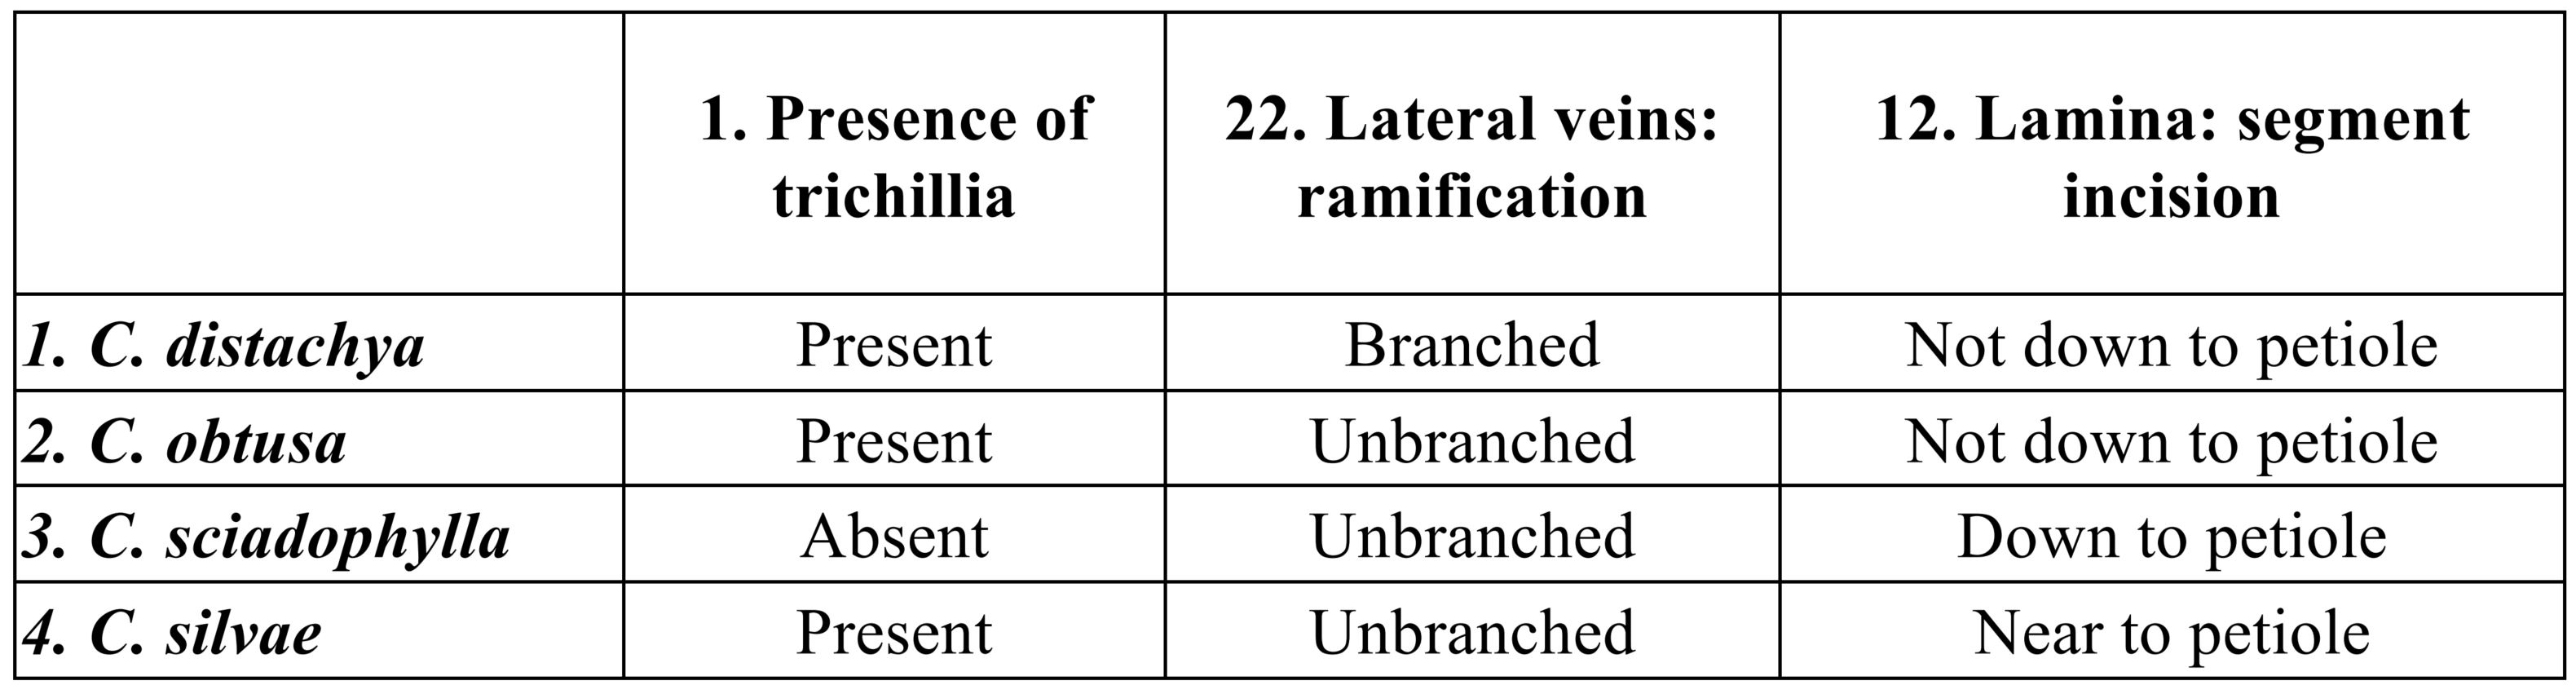
\includegraphics[width=1\linewidth]{figure/ex1} \end{center}

On transforme cette matrice en tableau disjonctif complet ou les états
deviennent des variables codées par des valeurs binaires avec 0 = Absent
et 1 = Présent ;

\begin{center}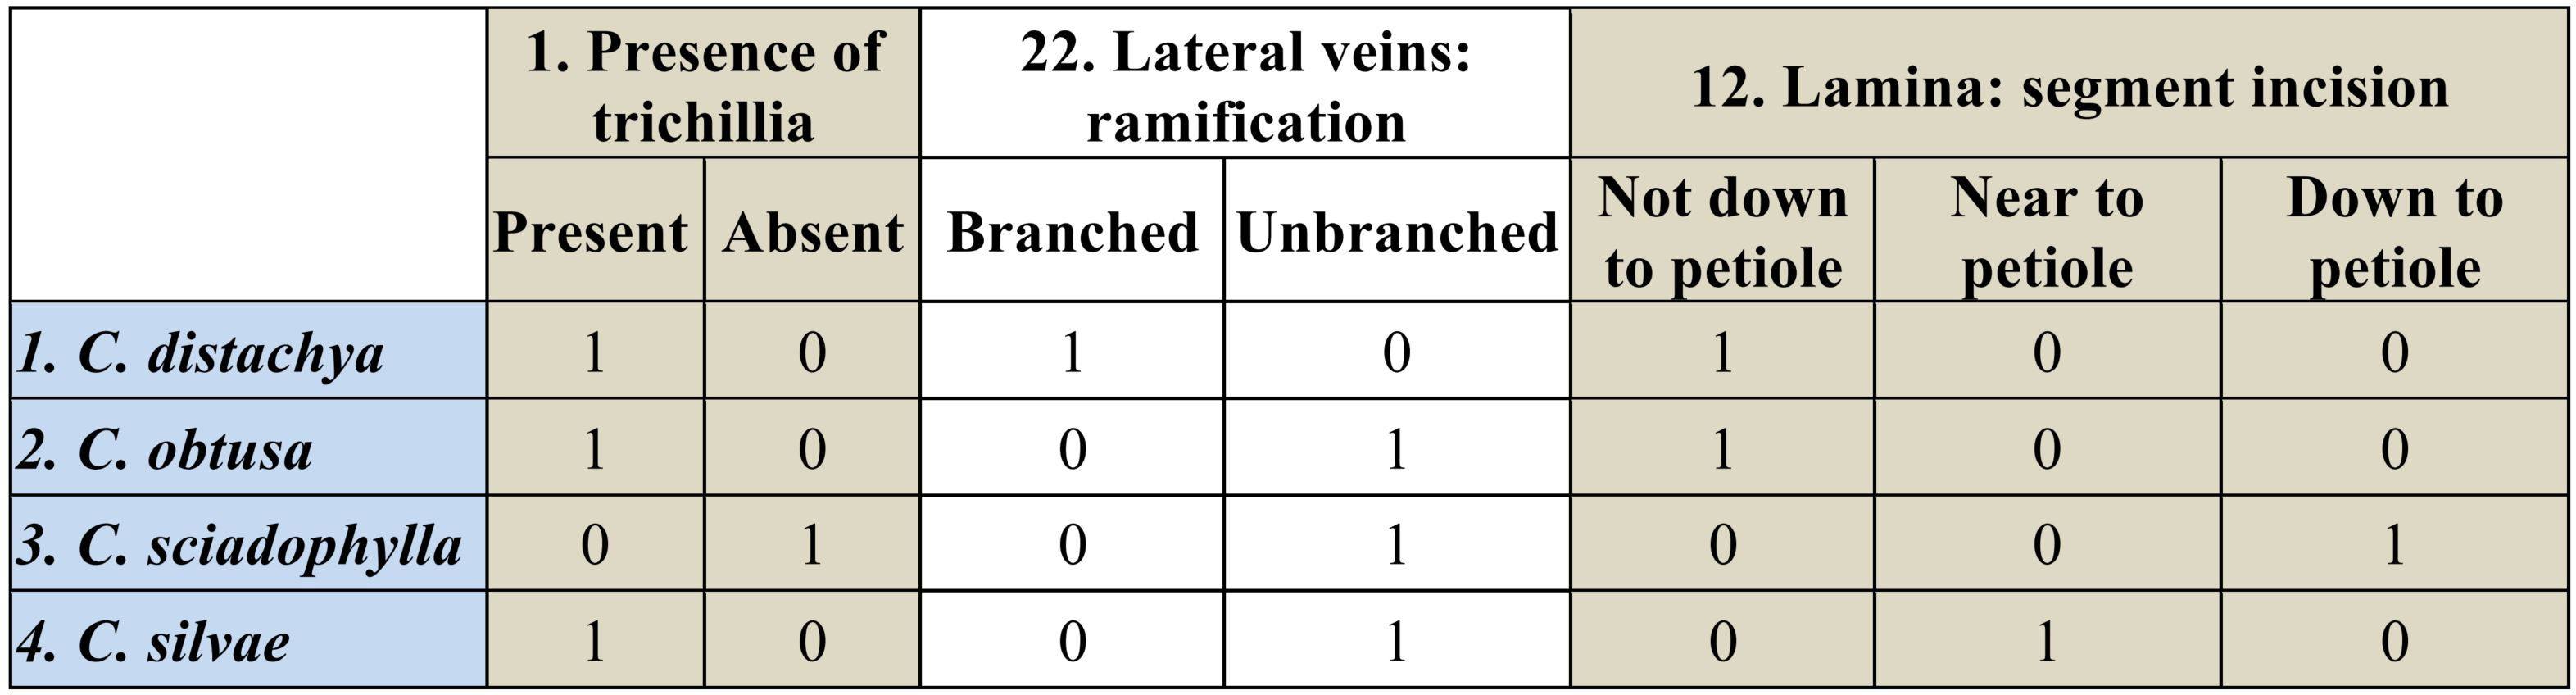
\includegraphics[width=1\linewidth]{figure/ex2} \end{center}

On compare alors deux à deux les espèces en calculant pour l'ensemble
des états définis :\\
a = le nombre d'états communs à deux espèces ;\\
b = le nombre d'états associés à l'espère i mais non associés à l'espèce
j ;\\
c = le nombre d'états associés à l'espère j mais non associés à l'espèce
i ;\\
d = le nombre d'états associés ni à l'espèce i, ni à l'espèce j ;

Dans notre cas avec 3 espèces, 6 comparaisons sont possibles deux à deux
:

\begin{center}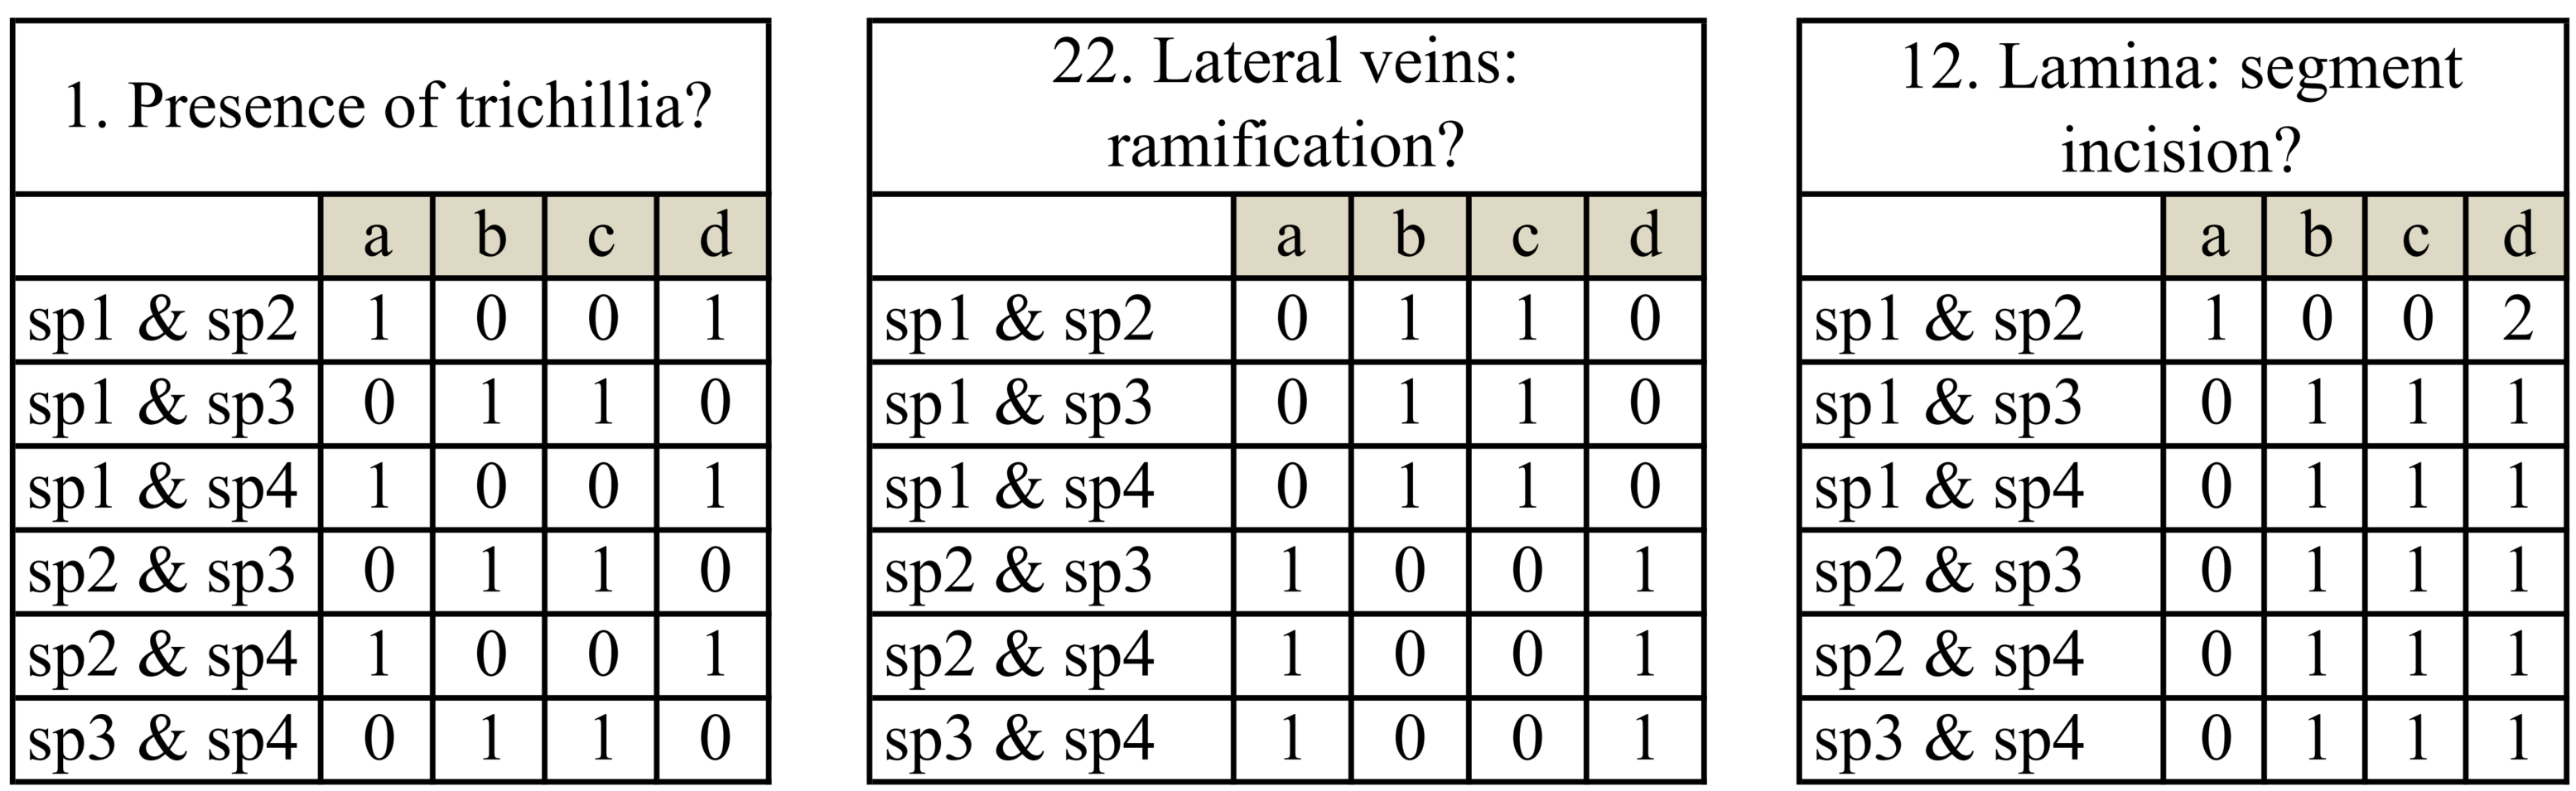
\includegraphics[width=1\linewidth]{figure/ex3} \end{center}

Pour chaque paire d'espèces, les indices sont calculés de la manière
suivante : \textbf{(i) L'indice de Jaccard} est un coefficient
d'association connu pour étudier la dissimilarité entre objets pour des
données binaires de présence-absence : \[d_{Jaccard}=\frac{b+c}{a+b+c}\]
\textbf{(ii) L'indice de Sokal et Michener} est calculé suivant la
formule suivante : \[d_{SM}=\frac{b+c}{a+b+c+d}\] Dans ce cas,
l'ensemble des états est pris en compte, y compris ceux qui ne sont
associé à aucune des espèces considérées.\\
\textbf{(iii) L'indice Xper\textsuperscript{2}} est basé sur
l'incompatibilité entre descriptions. Deux espèces sont incompatibles
(ou dissimilaires / discriminées) pour un descripteur s'ils n'ont aucun
état de caractère possible en commun \(a = 0\).\\
Formule : \(d_{Xper} = 1\) si \(a = 0\) ; sinon \(d_{Xper} = 0\)

\begin{center}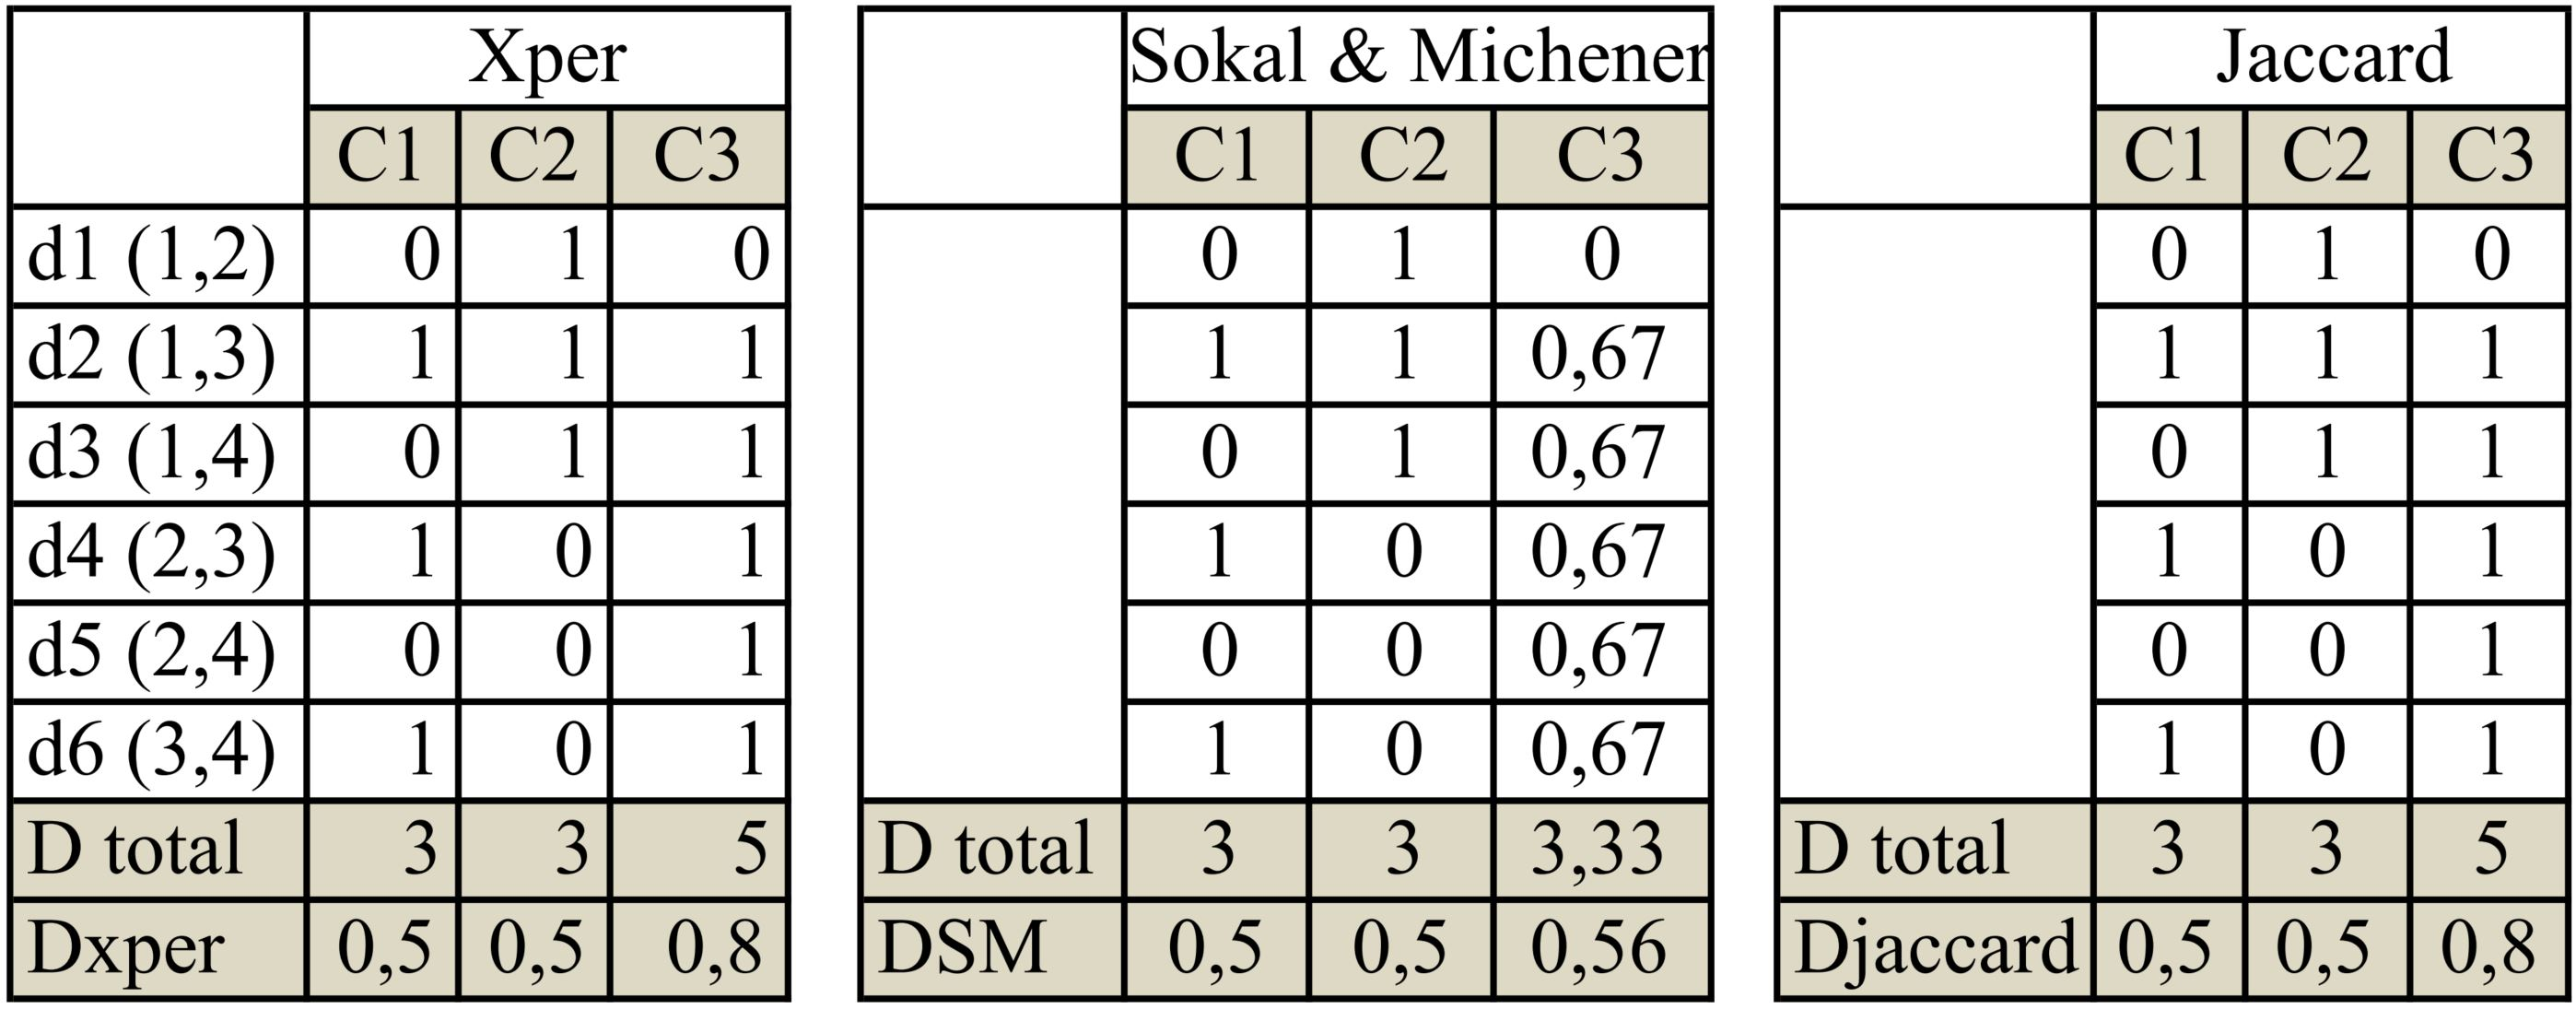
\includegraphics[width=1\linewidth]{figure/ex4} \end{center}

\subsubsection{Classification hiérarchique des
espèces}\label{classification-hierarchique-des-especes}

J'ai travaillé à partir d'une matrice de caractères comprenant le
tableau disjonctif des caractères qualitatifs et les minimas et maximas
des caractères continus. Une première étape a été de trouver une
solution pour les valeurs manquantes.\\
- Depuis la parution de l'ouvrage de B\&FR2005 de nouvelles observations
ont été faîte (photos, herbiers) et j'ai pu pour \emph{C. silvae} par
exemple renseigner des valeurs manquantes.\\
- Lorsque une seule espèce ne possédait pas d'information pour un
caractère avec peu d'état, j'ai mis la valeur 1 par défaut stipulant
ainsi que l'espèce peut potentiellement présenter tous les états.\\
- J'ai enlevé des variables concernant les minimas. En effet une
longueur de pétiole minimale n'a pour moi que peu de sens puisque cela
dépend des stades de développement échantillonnés.

Enfin, lorsque rien n'était possible, j'ai privilégié l'abandon d'un
caractère plutôt que l'abandon d'une espèce. J'ai ainsi travaillé sur
une matrice de 61 lignes et 138 colonnes (dont 117 variables binaires et
21 variables continues). J'ai effectué 3 types de classification
hiérarchique. La première repose sur une analyse mixte des variables
binaires et des variables continues. La métrique choisie pour calculer
la distance sur les variables binaires est celle de Dice
\citeyearpar{Dice1945} tandis que c'est celle de Gower
\citeyearpar{Gower1971} choisie pour les variables continues. La
classification hiérachique est construite selon la méthode UPGMA
(\textbf{U}nweighted \textbf{P}air \textbf{G}roup \textbf{M}ethod with
\textbf{A}rithmetic Mean). Pour les deux suivantes, j'ai travaillé
séparément soit sur les variables binaires (Fig. \ref{fig:fig10b},
indice de Dice, méthode UPGMA), soit sur les variables continues (Fig.
\ref{fig:fig10c}, distance euclidienne, méthode UPGMA) ce qui a permis
de faire un test de bootstrap pour vérifier la robustesse des différents
nœuds de l'arbre (1000 répétitions). Les analyses ont été effectuées
avec le logiciel PAST (PAlaeontological STatistics) \citep{Clarke1993}

\subsection{Etude de cas en Guyane
française}\label{etude-de-cas-en-guyane-francaise}

Finalement, cette clef a été testée sur le terrain en Guyane Française
(Fig. \ref{fig:fig4}) ou 7 espèces de \emph{Cecropia} sont censées être
présentes : \emph{C. obtusa, C. sciadophylla, C. palmata, C. distachya,
C. silvae, C. latiloba} et \emph{C. granvilleana} (Boggan et al. 1997
données de l'herbier de Cayenne). J'ai essentiellement prospecté (i)
dans l'ouest de la Guyane, sur la route St-Laurent du Maroni-Apatou qui
a été récemment ouverte en 2006, (ii) dans l'ouest, sur la piste
forestière de la Mataroni sur la route Régina-St-Georges et (iii) vers
Iracoubi, sur la piste forestière de Counami. J'ai eu l'occasion
d'observer toutes les espèces en dehors de \emph{C. granvilleana}. Il
n'existe que 4 échantillons au monde pour cette espèce qui pousse sur
les inselbergs. Je l'ai cherché à Savanne-Roche virginie
(N4°11'03,8'`W52°08'07,4'') sans succès. J'ai pu ainsi tester ma clef
multi-entrées sur de nombreux morphotypes et je présenterai les
limitations que j'ai rencontrées dans la partie « Résultats ». Ces
observations m'ont permis de mener une réflexion sur la mise au point de
protocole d'observation et de prise de vue photographique formaté pour
une prise de données pertinente et homogène par le plus grand nombre.




\begin{figure}[H]

{\centering 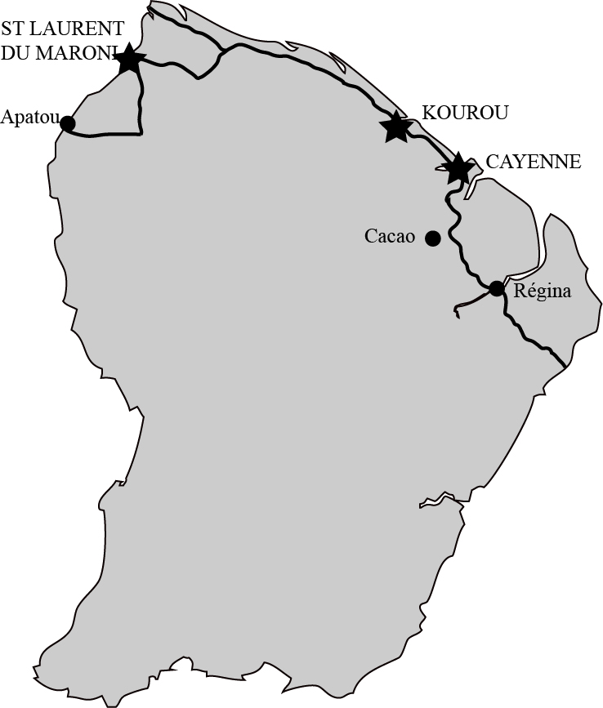
\includegraphics[width=0.7\linewidth]{figure/fig4} 

}

\caption{La carte de Guyane Française et la nouvelle route de Apatou à
Régina}\label{fig:fig4}
\end{figure}

\pagebreak

\section{Résultat}\label{resultat}

\subsection{\texorpdfstring{La base de donnée de
\emph{Cecropia}}{La base de donnée de Cecropia}}\label{la-base-de-donnee-de-cecropia}

A partir de l'ouvrage de B\&FR2005 j'ai retenu 59 caractères
morphométriques que j'ai divisé 9 grandes classes selon la partie de la
plante concernée : (i) le trichilium -- 9 caractères, (ii), le limbe --
16 caractères, (iii) le pétiole -- 3 caractères, (iv) la calyptre -- 6
caractères, (v) l'inflorescence mâle -- 7 caractères, (vi)
l'inflorescence femelle -- 7 caractères, (vii) la spathe -- 6
caractères, (viii) le fruit -- 3 caractères et (ix) la tige -- 2
caractères. A cela j'ai rajouté un 60ème caractère (qui constitue la
10ème classe) concernant la localisation géographique et qui est le
point d'entrée de la clef dichotomique de B\&FR2005. 39 caractères
correspondent à des variables catégorielles pour un total de 191 états.
Les 20 caractères restant correspondent à des variables numériques. 50
des caractères correspondent à ceux utilisés par B\&FR2005 dans leurs
clefs de début d'ouvrage. J'ai rajouté à cela 10 caractères à partir des
descriptions détaillées qu'ils ont fait pour chaque espèce et qu'ils
n'ont apparemment pas jugé utile d'utiliser comme caractères
discriminants (voir le détail en Annexe 2). L'ouvrage de B\&FR2005 ne
m'a pas permis de renseigner l'ensemble de ces caractères pour les 61
espèces et la matrice est renseignée à 77.46 \%.

\subsection{\texorpdfstring{Notice d'utilisation de la clef multi-entrée
: l'exemple de \emph{C.
distachya}}{Notice d'utilisation de la clef multi-entrée : l'exemple de C. distachya}}\label{notice-dutilisation-de-la-clef-multi-entree-lexemple-de-c.-distachya}

En mode \texttt{identification}, la clef que j'ai développée sous Xper2
se présente de la manière suivante (Fig. \ref{fig:fig5}): dans la
sous-fenêtre (A) se trouve la liste des caractères morphométriques. Il
est possible de les filtrer par groupes et de les classer selon les
valeurs des indices Xper, Jaccard ou Sokal \& Michener. J'ai rajouté un
groupe appelé `je propose' avec les caractères que j'ai jugé comme les
plus pertinents quelque soit la partie de la plante qu'ils concernent
(le choix de ces caractères sera discuté par la suite). Dans la
sous-fenêtre (B), se trouvent les différents états possibles du
caractère sélectionné. J'ai illustré la plupart des caractères et leurs
états possibles avec des dessins ou des photographies (D) et j'y ai
associé une définition dans la majorité des cas (C) Dans la sous-fenêtre
(E) figure la liste des 61 espèces qui sont conformes aux critères
sélectionnés. Dans la sous-fenêtre (F), figurent les espèces qui ne sont
pas conformes aux critères sélectionnés.








\begin{figure}[H]

{\centering 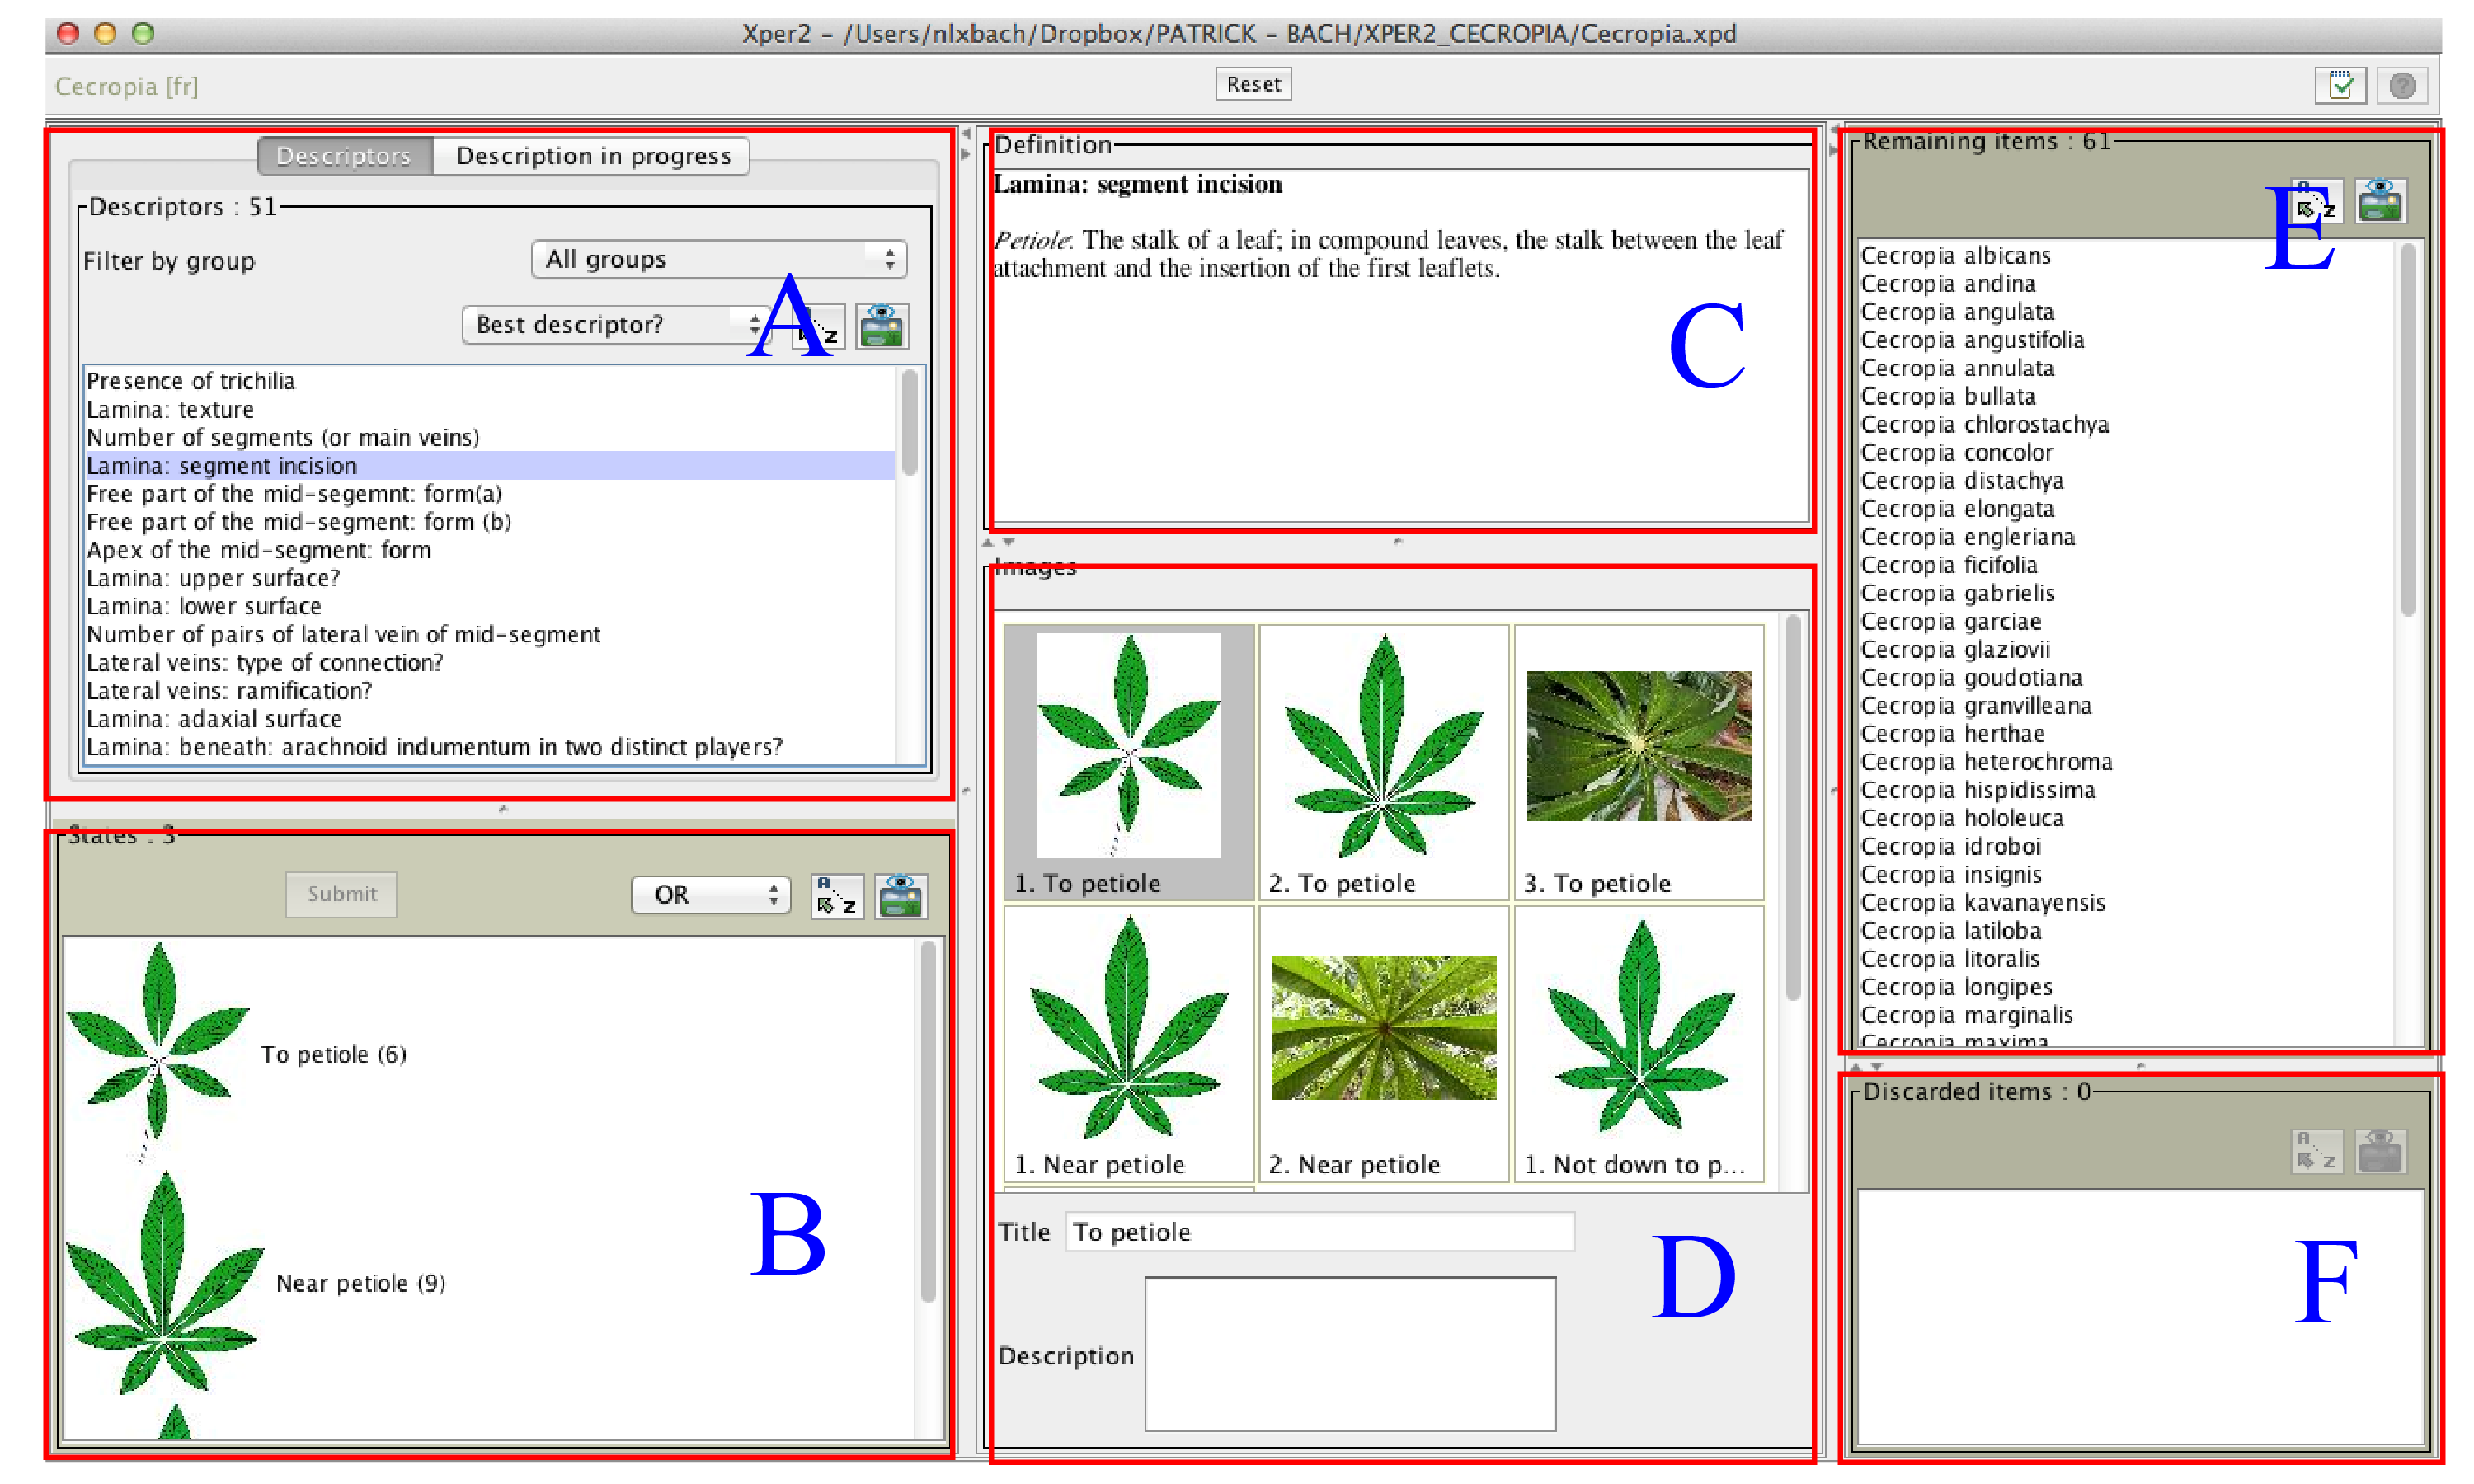
\includegraphics[width=0.9\linewidth]{figure/fig5} 

}

\caption{: Interface d'indentification du logiciel XPER2\_Cecropia (A.
Liste des caractères pertinants pour l'identification; B. Liste des
états correspondants au caractère sélectionné en A; C. Définitions des
caractères; D. Illustrations des états de caractères; E. Liste des
taxons correspondants aux états de caractères sélectionnés; F. Liste des
taxons qui ne correspondent pas aux états de caractère choisis)}\label{fig:fig5}
\end{figure}

En double-cliquant sur une espèce on accède à une fiche détaillée avec
(i) la description textuelle de B\&FR2005, (ii) un ensemble
d'illustrations judicieusement choisies dans la photothèque que j'ai
construite et (iii) la description formatée pour l'ensemble des
caractères renseignés dans la matrice et rassemblés selon les groupes
définis (Fig. \ref{fig:fig6}). Si l'espèce sur laquelle on clique se
trouve parmi la liste de celles qui ne sont pas retenues dans la
description courante (sous-fenêtre F) alors les caractères qui ne sont
pas en accord avec les choix effectués apparaissent en rouge. En
sélectionnant plusieurs espèces dans les fenêtres (E) ou (F) et en
faisant clique-droit \textgreater{} \texttt{Comparaison} on visualise la
matrice de caractère avec les critères qui sont discriminants pour les
espèces sélectionnées. Avec clique-droit \textgreater{}
\texttt{Particularité(s)} ont obtient une liste des états possédés
uniquement par les espèces choisies.






\begin{figure}[H]

{\centering 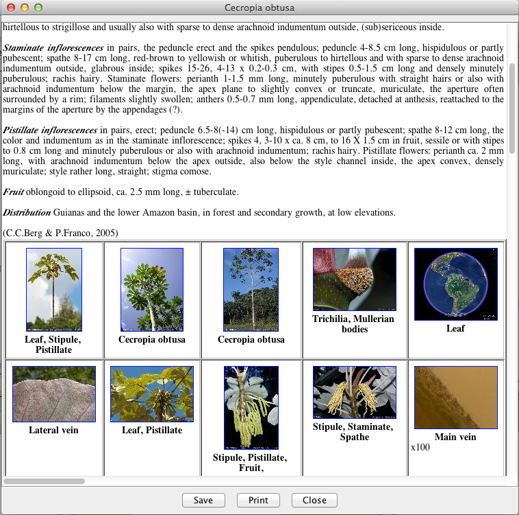
\includegraphics[width=0.7\linewidth]{figure/fig6} 

}

\caption{: Une fiche détaillée avec (i) la description textuelle de
B\&FR2005, (ii) un ensemble d'illustrations et (iii) la description
formatée pour l'ensemble des caractères renseignés dans la matrice et
rassemblés selon les groupes définis.}\label{fig:fig6}
\end{figure}

En l'état actuel, 470 images et illustrations sont associées aux
différentes descriptions (caractères, états, espèces). A titre d'exemple
d'utilisation, je prendrais la planche d'herbier présentée Fig.
\ref{fig:fig7}. Sur cette photographie, \textbf{13 caractères}
morphométriques sont observables:

\begin{enumerate}
\def\labelenumi{\arabic{enumi})}
\tightlist
\item
  L'inflorescence mâle comporte 10 épis ; En renseignant \textbf{« 35.
  Staminate spikes: number» = 10} alors 34 espèces sont exclues. 27
  espèces restent en course et sont potentiellement celles que l'on
  cherche à identifier.
\item
  Le nombre de lobes est de 8 ; En renseignant \textbf{« 11. Number of
  segment (or main vein) » = 8} alors 8 espèces supplémentaires sont
  exclues et 19 espèces restent en course.
\item
  Le plus grand épi possède un diamètre de 3 mm ; En renseignant
  \textbf{« 40. Staminate spikes: maximal diameter» = 3} alors 6 espèces
  supplémentaires sont exclues et 13 espèces restent en course.
\item
  Les nervures secondaires sont connectées ensembles sur la marge du
  limbe ; En renseignant \textbf{« 21. Lateral veins: type of connection
  » \textgreater{} `Marginally'} alors 6 espèces supplémentaires sont
  exclues et 7 espèces restent en course.
\item
  Les nervures secondaires portent des nervures tertiaires ; Ce
  caractère n'est pourtant visible que sur le lobe situé le long du
  pétiole ce qui pourrait être une sorte d'anomalie (en fait, dans le
  cas de cette espèce, c'est plutôt le fait que ce caractère soit si peu
  marqué qui en est une) ; En renseignant \textbf{« 22. Lateral veins:
  ramification » \textgreater{} `Branched'} alors deux espèces
  supplémentaires sont exclues. Face à l'ambigüité du spécimen nous
  décidons de ne pas renseigner ce critère.
\item
  Le pétiole mesure 22.4 cm ; En renseignant \textbf{« 26. Petiole :
  length » = 22.4} alors deux espèces supplémentaires sont exclues et 5
  restent en course
\item
  Le plus grand épi mesure environ 8.5 cm de longueur ; En renseignant
  \textbf{« 39. Staminate spikes: maximal length» = 8.5} alors une
  nouvelle espèce est écartée. 4 espèces restent en course.
\item
  Les lobes sont entiers dans le sens ou ils ne sont pas redécoupé
  eux-mêmes en \texttt{feuille\ de\ chêne} ; En renseignant \textbf{«
  14. Free part of the mid-segment: form(a)'' \textgreater{} `Entire'}
  alors une nouvelle espèce est écartée et 3 espèces restent en course.
\item
  La partie libre du lobe principal est plutôt d'une forme obovale,
  c'est à dire que la largeur maximale se trouve au delà de la partie
  médiane ; En renseignant \textbf{« 16. Free part of the mid-segment:
  form(b)'' \textgreater{} `Obovate'} alors une nouvelle espèce est
  écartée et 2 espèces restent en course.
\end{enumerate}




\begin{figure}[H]

{\centering 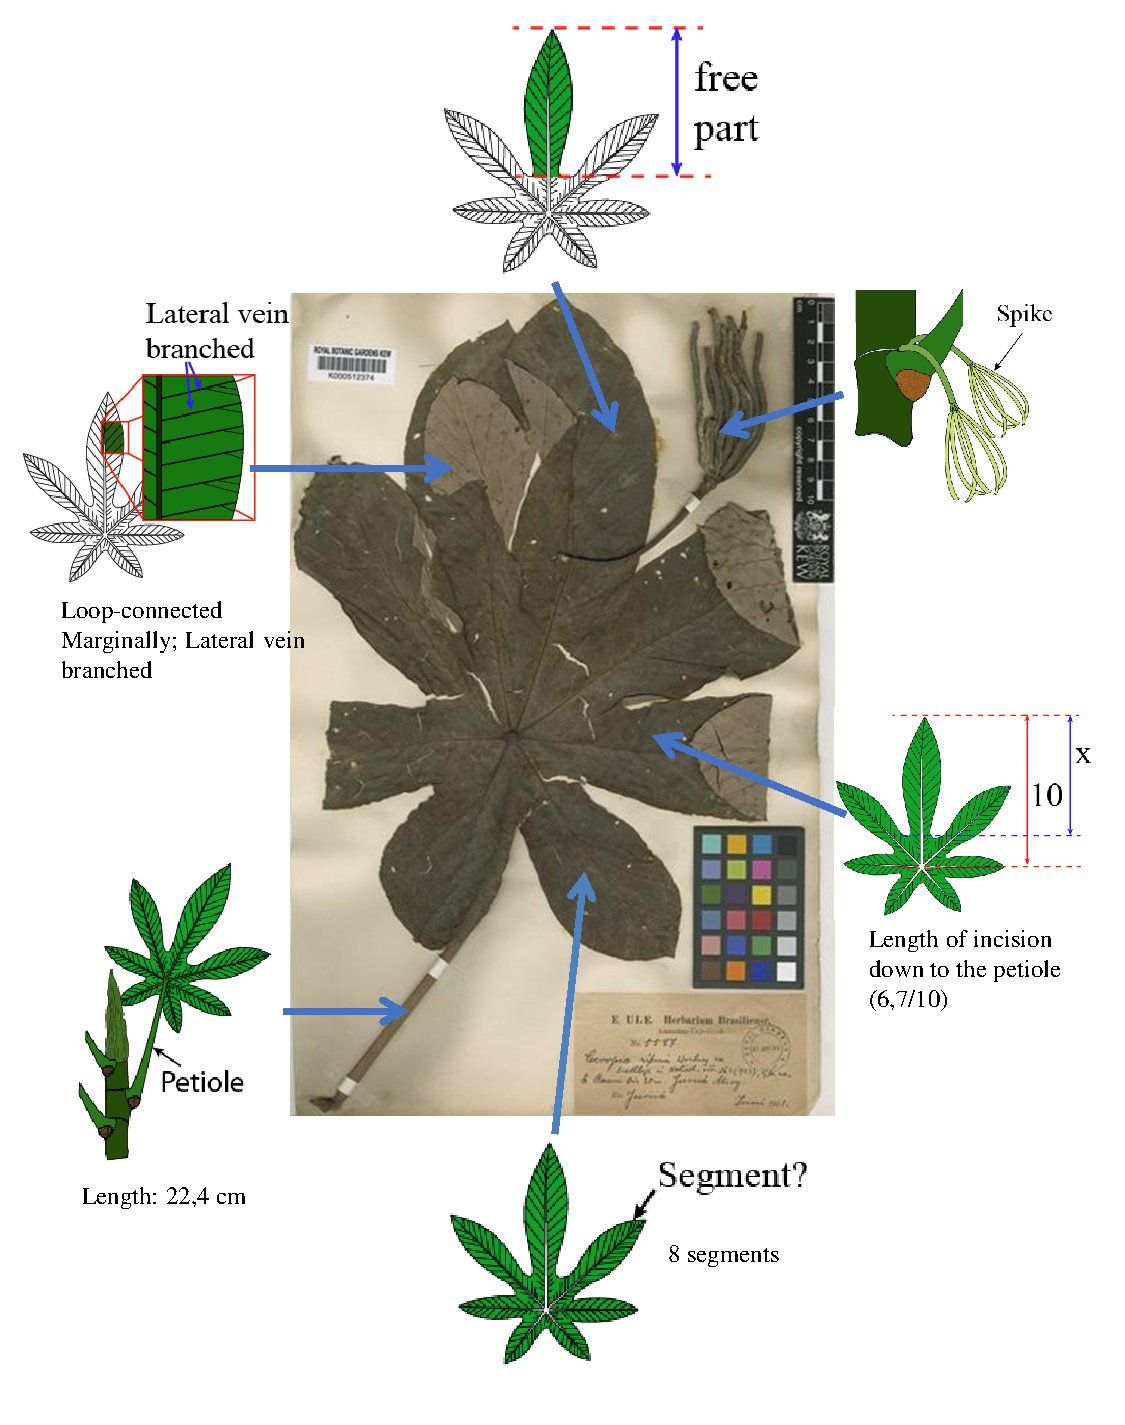
\includegraphics[width=1\linewidth]{figure/fig7} 

}

\caption{Photographie d'échantillon d'herbier \emph{C. distachya}
(KEW-K000512374). 13 caractères morphométriques sont observables.}\label{fig:fig7}
\end{figure}

A ce stade, les 4 derniers critères observables ne permettent pas
d'affiner la recherche : 10. On compte environ 16 paires de nervures
secondaires sur la partie libre du lobe principal : « 20. Number of
pairs of lateral veins in the mid-segment » = 16 ; 11. Les lobes sont
soudés à leur base et ne sont pas libre jusqu'à leur insertion sur le
pétiole : \textbf{« 12. Lamina: segment incision » \textgreater{} `Not
down to petiole'}; 12. Le lobe principal mesure environ 22.2 cm. La
partie soudée représente 7.4 cm tandis que la partie libre représente
14.8 cm. La partie libre représente ainsi 6.7/10 de la longueur totale
du lobe : \textbf{« 13. Free part of the mid-segment length/Total
mid-segment length ratio» = 6.7}; 13. Le pédoncule de l'inflorescence
mesure environ 9.4 cm de long: \textbf{« 38. Staminate inflorescence:
peduncle length » = 9.4}.

Les deux espèces sont \emph{C. distachya} et \emph{C. obtusifolia} (Fig.
\ref{fig:fig8}). Notons qu'à ce stade le critère \textbf{« 22. Lateral
veins: ramification? »} n'est pas discriminant puisque ces deux espèces
sont censées avoir des nervures tertiaires. En sélectionnant les deux
espèces et en faisant clique-droit \textgreater{} \texttt{comparaison}
nous pouvons voir les critères qui permettent de les séparer. Seul le
type de stigmate ne laisse aucune ambigüité mais il n'est
malheureusement pas observable sur cet échantillon mâle. Avec cet unique
échantillon, il est donc impossible de trancher entre ces deux espèces.
Par contre, l'étiquette indique que ce spécimen a été collecté au Brésil
sur le Rio Juruá un des principaux affluents de l'amazone dans l'état de
l'Amazonas. En choisissant le critère de la position géographique :
\textbf{« 60. Location » \textgreater{} `Amazonian Brazil'} alors une
espèce unique est sélectionnée : \emph{C. distachya} ce qui est
effectivement la détermination attribuée à cet échantillon (\emph{C.
riparia} étant un synonyme de \emph{C. distachya}). A noter que dans le
processus que nous avons décrit ci-dessus, si la position géographique
avait été entrée en tant que premier critère, l'espèce aurait été
identifié dès que le quatrième critère aurait été renseigné (\textbf{«
21. Lateral veins: type of connection? »}).





\begin{figure}[H]

{\centering 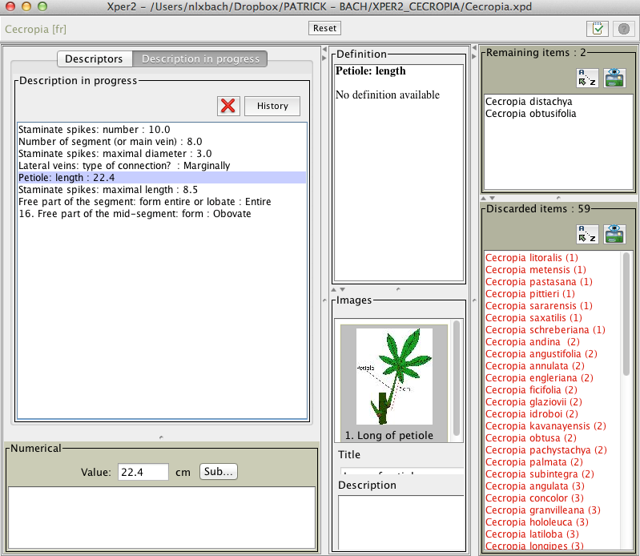
\includegraphics[width=1\linewidth]{figure/fig8} 

}

\caption{: XPER2 propose 2 espèces \emph{C. distachya} et \emph{C.
obtusifolia} qui ont les caractères compatibles avec les 13 caractères
observés sur l'échantillon d'herbier montré Fig. \ref{fig:fig7}}\label{fig:fig8}
\end{figure}

Comparons cette démarche avec celle suivie dans B\&FR2005 au travers de
la clef dichotomique (Fig. \ref{fig:fig9} ) : En dehors du critère
géographique qui est le premier point d'entrée, on notera que : (i) Pour
le critère n°2, les trichilias ne sont pas observables sur notre
échantillon mais le fait que les lobes ne sont pas découpés jusqu'à leur
insertion sur le pétiole nous permet de faire un choix ; (ii) Le dernier
critère relatif au statut érigé ou pendant de l'inflorescence n'est pas
observable. En suivant la clef de B\&FR2005 deux espèces potentielles
seraient retenues : \emph{C. palmata} et \emph{C. distachya}. Dans notre
identification par Xper2, \emph{C. palmata} avait été écarté car chez
cette espèce (i) le nombre d'épis mâles par inflorescence varie entre 4
et 6 et (ii) Le diamètre des épis mâle varie entre 8 et 18 cm. Pour cet
exemple, nous arrivons donc à identifier l'espèce avec 5 critères (dont
la position géographique) tandis que avec l'utilisation de cette clef
dichotomique, le renseignement de 7 critères nous amène à un dilemme
entre deux espèces.





\begin{figure}[H]

{\centering 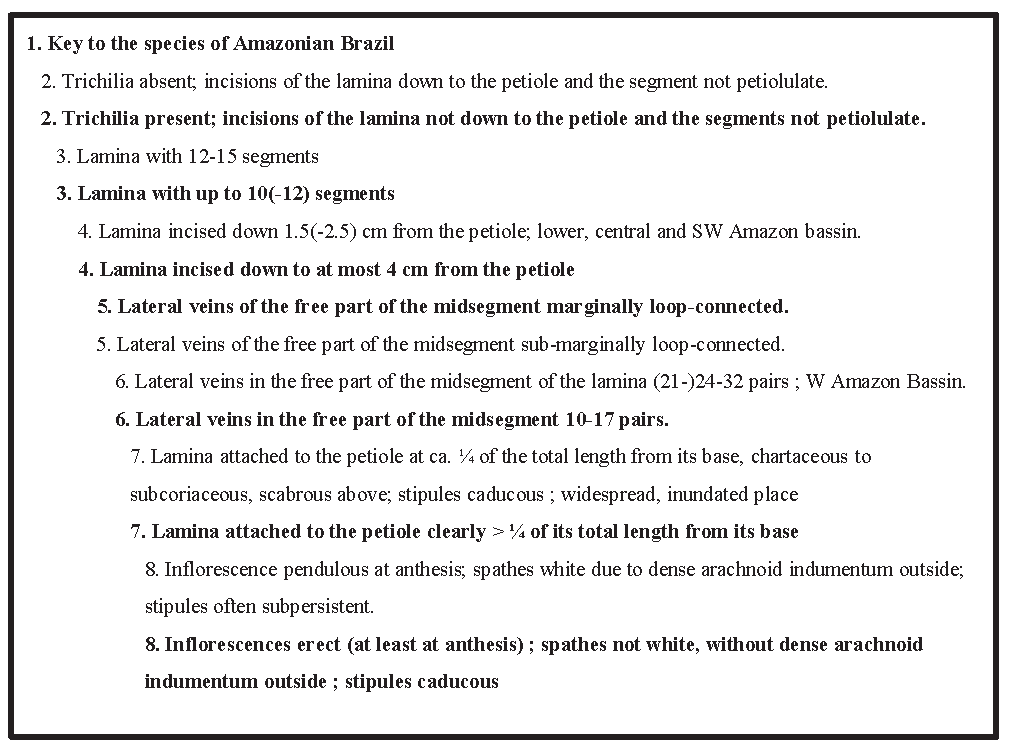
\includegraphics[width=1\linewidth]{figure/fig9} 

}

\caption{: XPER2 propose 2 espèces \emph{C. distachya} et \emph{C.
obtusifolia} qui ont les caractères compatibles avec les 13 caractères
observés sur l'échantillon d'herbier montré Fig. \ref{fig:fig7}}\label{fig:fig9}
\end{figure}

\subsection{Analyse discriminante des caractères selon différents
indices de
dissimilarité}\label{analyse-discriminante-des-caracteres-selon-differents-indices-de-dissimilarite}

Les différents indices de dissimilarité utilisés n'ont de sens que
lorsqu'ils traitent des caractères de même type. Nous avons donc
travaillé sur deux groupes de caractères selon qu'ils étaient numériques
ou catégoriels

En ce qui concerne les caractères numériques (Tab. \ref{tab:tab1}), les
indices de Jaccard et de Sokal \& Michener ne montrent aucune
différence. Si l'on prends comme seuil, la moitié de l'indice maximal, 9
variables sont sélectionnées avec l'indice Xper (au delà du seuil de
0.28 ; en bleu). Ces 9 variables sont également sélectionnées avec les
indices de Jaccard / Sokal \& Michener (au delà du seuil de 0.50) ainsi
que 6 variables supplémentaires (en vert). Parmi ces critères, « 26.
Petiole: length » et « 46. Pistillate spikes: maximal diameter» sont des
critères non utilisé par B\&FR2005 dans leurs clefs dichotomiques et
pourtant pertinents.

En ce qui concerne les caractères catégoriels (Tab. \ref{tab:tab2}), si
l'on prends comme seuil, la moitié de l'indice maximal, 11 variables
sont sélectionnées avec l'indice Xper (au delà du seuil de 0.26 ; en
bleu). Ces 9 variables sont également sélectionnées avec les indices de
Jaccard et de Sokal \& Michener (au delà du seuil de 0.40 et 0.25
respectivement). L'indice de Jaccard amène à considérer 9 variables
supplémentaires (en vert). L'indice de Sokal \& Michener amène à
considérer 11 variables supplémentaires, dont deux non retenues par
l'indice de Jaccard (en orange). Parmi ces critères, « 57. Fruit:
surface», « 56. Fruit: form» et « 17. Apex of the mid-segment: form »
sont des critères non utilisés par B\&FR2005 dans leurs clefs
dichotomiques et pourtant pertinents.

La plupart des ces critères sont observables sur un minimum de
photographie que l'on peut prendre aisément sur le terrain. Dans
l'Annexe 3, je propose un ensemble de vues (compilées à partir de
différentes espèces) que pourraient prendre n'importe quel néophyte et
qui permettrait à priori d'identifier l'espèce. Les caractères
importants et qui restent difficile à saisir sur une photographie sans
un examen attentif du spécimen sont « 48. Stigma: type », « 57. Fruit:
surface », « 10. Lamina: texture » (ex : coriace, chartacée), « 56.
Fruit: form » et « 18. Lamina: upper surface « (ex : glabre,
pubérulant). En plus de ce protocole photographique que je propose, je
propose pour des contributeurs plus confirmés une feuille type
comportant les caractères à observer et à renseigner ainsi qu'une
illustration de ces caractères (Annexe 4). Les critères concernant les
poils sont réduit à la simple observation d'un indumentum arachnoïde sur
le pétiole ; en effet la terminologie concernant la pilosité adoptée par
B\&FR2005 comporte de nombreux états dont nous n'avons pas toujours
saisi les nuances.

\begin{table}[!h]

\caption{\label{tab:tab1}Liste des caractères numériques et leur indice de dissimilarité calculés dans XPER2. Les valeurs en gras indiquent les valeurs maximales par indice utilisé}
\centering
\resizebox{\linewidth}{!}{
\begin{tabular}[t]{>{\raggedright\arraybackslash}p{25em}lll}
\toprule
\textbf{Liste caracterès} & \textbf{XPER} & \textbf{Jaccard} & \textbf{Sokal\&Michener}\\
\midrule
\textcolor[HTML]{0072ff}{35. Staminate spikes: number} & \textcolor[HTML]{0072ff}{\textbf{1016/1830 (0.56)}} & \textcolor[HTML]{0072ff}{\textbf{1827/1830 (1.0)}} & \textcolor[HTML]{0072ff}{\textbf{1827/1830 (1.0)}}\\
\textcolor[HTML]{0072ff}{20. Number of pairs of lateral veins in the mid-segment} & \textcolor[HTML]{0072ff}{999/1830 (0.55)} & \textcolor[HTML]{0072ff}{\textbf{1826/1830 (1.0)}} & \textcolor[HTML]{0072ff}{\textbf{1826/1830 (1.0)}}\\
\textcolor[HTML]{0072ff}{11. Number of segment (or main vein)} & \textcolor[HTML]{0072ff}{941/1830 (0.51)} & \textcolor[HTML]{0072ff}{\textbf{1825/1830 (1.0)}} & \textcolor[HTML]{0072ff}{\textbf{1825/1830 (1.0)}}\\
\textcolor[HTML]{0072ff}{13. Free part of the mid-segment length/Total mid-segment length ratio} & \textcolor[HTML]{0072ff}{640/1485 (0.43)} & \textcolor[HTML]{0072ff}{1374/1485 (0.93)} & \textcolor[HTML]{0072ff}{1374/1485 (0.93)}\\
\textcolor[HTML]{0072ff}{40. Staminate spikes: maximal diameter} & \textcolor[HTML]{0072ff}{707/1830 (0.39)} & \textcolor[HTML]{0072ff}{1272/1830 (0.7)} & \textcolor[HTML]{0072ff}{1272/1830 (0.7)}\\
\addlinespace
\textcolor[HTML]{0072ff}{29. Stipule: length} & \textcolor[HTML]{0072ff}{684/1830 (0.37)} & \textcolor[HTML]{0072ff}{\textbf{1825/1830 (1.0)}} & \textcolor[HTML]{0072ff}{\textbf{1825/1830 (1.0)}}\\
\textcolor[HTML]{0072ff}{54. Staminate spathe: length} & \textcolor[HTML]{0072ff}{586/1830 (0.32)} & \textcolor[HTML]{0072ff}{1481/1830 (0.81)} & \textcolor[HTML]{0072ff}{1481/1830 (0.81)}\\
\textcolor[HTML]{0072ff}{42. Pistillate spikes: number} & \textcolor[HTML]{0072ff}{543/1830 (0.3)} & \textcolor[HTML]{0072ff}{987/1830 (0.54)} & \textcolor[HTML]{0072ff}{987/1830 (0.54)}\\
\textcolor[HTML]{0072ff}{39. Staminate spikes: maximal length} & \textcolor[HTML]{0072ff}{534/1830 (0.29)} & \textcolor[HTML]{0072ff}{\textbf{1824/1830 (1.0)}} & \textcolor[HTML]{0072ff}{\textbf{1824/1830 (1.0)}}\\
\textcolor[HTML]{0a7502}{44. Pistillate inflorescence: peduncle length} & 496/1830 (0.27) & \textcolor[HTML]{0a7502}{\textbf{1824/1830 (1.0)}} & \textcolor[HTML]{0a7502}{\textbf{1824/1830 (1.0)}}\\
\addlinespace
\textcolor[HTML]{0a7502}{53. Staminate spathe: length} & 448/1830 (0.24) & \textcolor[HTML]{0a7502}{1480/1830 (0.81)} & \textcolor[HTML]{0a7502}{1480/1830 (0.81)}\\
\textcolor[HTML]{0a7502}{38. Staminate inflorescence: peduncle length} & 359/1830 (0.2) & \textcolor[HTML]{0a7502}{1705/1830 (0.93)} & \textcolor[HTML]{0a7502}{1705/1830 (0.93)}\\
41. Staminate spikes: maximal stipe length & 290/1830 (0.16) & 858/1830 (0.47) & 858/1830 (0.47)\\
\textcolor[HTML]{0a7502}{46. Pistillate spikes: maximal diameter} & 282/1830 (0.15) & \textcolor[HTML]{0a7502}{1763/1830 (0.96)} & \textcolor[HTML]{0a7502}{1763/1830 (0.96)}\\
55. Fruit: length & 256/1830 (0.14) & 433/1830 (0.24) & 433/1830 (0.24)\\
\addlinespace
\textcolor[HTML]{0a7502}{45. Pistillate spikes: maximal length} & 243/1830 (0.13) & \textcolor[HTML]{0a7502}{1763/1830 (0.96)} & \textcolor[HTML]{0a7502}{1763/1830 (0.96)}\\
\textcolor[HTML]{0a7502}{26. Petiole: length} & 172/1830 (0.09) & \textcolor[HTML]{0a7502}{1822/1830 (1.0)} & \textcolor[HTML]{0a7502}{1822/1830 (1.0)}\\
59. Tree: height & 0/1830 (0.0) & 465/1830 (0.25) & 465/1830 (0.25)\\
47. Pistillate spikes: maximal stipe length & 7/1830 (0.0) & 35/1830 (0.02) & 35/1830 (0.02)\\
02. Müllerian bodies: length & 0/1540 (0.0) & 0/1540 (0.0) & 0/1540 (0.0)\\
\bottomrule
\end{tabular}}
\end{table}

\begingroup\fontsize{8}{10}\selectfont

\begin{longtable}[t]{>{\raggedright\arraybackslash}p{25em}lll}
\caption{\label{tab:tab2}Liste des caractères catégoriels et leur indice de dissimilarité calculés dans XPER2. Les valeurs en gras indiquent les valeurs maximales par indice utilisé.}\\
\toprule
\textbf{Liste caracterès} & \textbf{XPER} & \textbf{Jaccard} & \textbf{Sokal\&Michener}\\
\midrule
\endfirsthead
\caption[]{\label{tab:tab2}Liste des caractères catégoriels et leur indice de dissimilarité calculés dans XPER2. Les valeurs en gras indiquent les valeurs maximales par indice utilisé. \textit{(continued)}}\\
\toprule
\textbf{Liste.caracteres} & \textbf{XPER} & \textbf{Jaccard} & \textbf{Sokal.Michener}\\
\midrule
\endhead
\
\endfoot
\bottomrule
\endlastfoot
\textcolor[HTML]{0072ff}{48. Stigma: type} & \textcolor[HTML]{0072ff}{\textbf{959/1830 (0.52)}} & \textcolor[HTML]{0072ff}{1134/1830 (0.62)} & \textcolor[HTML]{0072ff}{652/1830 (0.36)}\\
\textcolor[HTML]{0072ff}{32. Stipule: indumentum on the inner part} & \textcolor[HTML]{0072ff}{931/1830 (0.51)} & \textcolor[HTML]{0072ff}{1265/1830 (0.69)} & \textcolor[HTML]{0072ff}{435/1830 (0.24)}\\
\textcolor[HTML]{0072ff}{49. Spathe: color} & \textcolor[HTML]{0072ff}{751/1830 (0.41)} & \textcolor[HTML]{0072ff}{\textbf{1467/1830 (0.8)}} & \textcolor[HTML]{0072ff}{785/1830 (0.43)}\\
\textcolor[HTML]{0072ff}{16. Free part of the mid-segment: form} & \textcolor[HTML]{0072ff}{716/1830 (0.39)} & \textcolor[HTML]{0072ff}{1366/1830 (0.75)} & \textcolor[HTML]{0072ff}{675/1830 (0.37)}\\
\textcolor[HTML]{0072ff}{22. Lateral veins: ramification} & \textcolor[HTML]{0072ff}{624/1830 (0.34)} & \textcolor[HTML]{0072ff}{899/1830 (0.49)} & \textcolor[HTML]{0072ff}{\textbf{899/1830 (0.49)}}\\
\addlinespace
\textcolor[HTML]{0072ff}{57. Fruit: surface} & \textcolor[HTML]{0072ff}{604/1830 (0.33)} & \textcolor[HTML]{0072ff}{1054/1830 (0.58)} & \textcolor[HTML]{0072ff}{875/1830 (0.48)}\\
\textcolor[HTML]{0072ff}{37. Staminate inflorescence: spike positions} & \textcolor[HTML]{0072ff}{580/1830 (0.32)} & \textcolor[HTML]{0072ff}{874/1830 (0.48)} & \textcolor[HTML]{0072ff}{874/1830 (0.48)}\\
\textcolor[HTML]{0072ff}{31. Stipule: indumentum on the outer part} & \textcolor[HTML]{0072ff}{547/1830 (0.3)} & \textcolor[HTML]{0072ff}{1395/1830 (0.76)} & \textcolor[HTML]{0072ff}{447/1830 (0.24)}\\
\textcolor[HTML]{0072ff}{50. Spathe: indumentum on the outer part} & \textcolor[HTML]{0072ff}{548/1830 (0.3)} & \textcolor[HTML]{0072ff}{1365/1830 (0.75)} & \textcolor[HTML]{0072ff}{468/1830 (0.26)}\\
\textcolor[HTML]{0072ff}{10. Lamina: texture} & \textcolor[HTML]{0072ff}{488/1830 (0.27)} & \textcolor[HTML]{0072ff}{995/1830 (0.54)} & \textcolor[HTML]{0072ff}{865/1830 (0.47)}\\
\addlinespace
\textcolor[HTML]{0072ff}{21. Lateral veins: type of connection} & \textcolor[HTML]{0072ff}{468/1830 (0.26)} & \textcolor[HTML]{0072ff}{723/1830 (0.4)} & \textcolor[HTML]{0072ff}{723/1830 (0.4)}\\
\textcolor[HTML]{0a7502}{56. Fruit: form} & 458/1830 (0.25) & \textcolor[HTML]{0a7502}{947/1830 (0.52)} & \textcolor[HTML]{0a7502}{768/1830 (0.42)}\\
\textcolor[HTML]{0a7502}{08. Trichilia: hair length} & 377/1540 (0.24) & \textcolor[HTML]{0a7502}{638/1540 (0.41)} & 370/1540 (0.24)\\
\textcolor{red}{36. Staminate inflorescence: peduncle position} & 378/1830 (0.21) & 633/1830 (0.35) & \textcolor{red}{633/1830 (0.35)}\\
\textcolor[HTML]{0a7502}{18. Lamina: upper surface} & 359/1830 (0.2) & \textcolor[HTML]{0a7502}{1265/1830 (0.69)} & \textcolor[HTML]{0a7502}{639/1830 (0.35)}\\
\addlinespace
\textcolor[HTML]{0a7502}{30. Stipule: color} & 331/1830 (0.18) & \textcolor[HTML]{0a7502}{1266/1830 (0.69)} & \textcolor[HTML]{0a7502}{613/1830 (0.34)}\\
\textcolor[HTML]{0a7502}{17. Apex of the mid-segment: form} & 338/1830 (0.18) & \textcolor[HTML]{0a7502}{967/1830 (0.53)} & \textcolor[HTML]{0a7502}{637/1830 (0.35)}\\
\textcolor[HTML]{0a7502}{28. Petiole: indumentum} & 309/1830 (0.17) & \textcolor[HTML]{0a7502}{1242/1830 (0.68)} & \textcolor[HTML]{0a7502}{460/1830 (0.25)}\\
12. Lamina: segment incision & 316/1830 (0.17) & 507/1830 (0.28) & 375/1830 (0.21)\\
\textcolor[HTML]{0a7502}{43. Pistillate inflorescence: position} & 260/1830 (0.14) & \textcolor[HTML]{0a7502}{722/1830 (0.39)} & \textcolor[HTML]{0a7502}{722/1830 (0.39)}\\
\addlinespace
01. Presence of trichilia & 255/1830 (0.14) & 395/1830 (0.22) & 395/1830 (0.22)\\
04. Trichilia: type & 135/1540 (0.09) & 327/1540 (0.21) & 327/1540 (0.21)\\
\textcolor{red}{06. Trichilia: form} & 115/1540 (0.07) & 507/1540 (0.33) & \textcolor{red}{507/1540 (0.33)}\\
09.Trichilia: hair color & 88/1485 (0.06) & 426/1485 (0.29) & 318/1485 (0.21)\\
19. Lamina: lower surface & 88/1830 (0.05) & \textcolor[HTML]{0a7502}{1066/1830 (0.58)} & \textcolor[HTML]{0a7502}{524/1830 (0.29)}\\
\addlinespace
33. Stipule:persistance and texture & 29/1830 (0.02) & 568/1830 (0.31) & \textcolor{red}{539/1830 (0.29)}\\
51. Spathe: indumentum on the inner part & 40/1830 (0.02) & \textcolor[HTML]{0a7502}{794/1830 (0.43)} & \textcolor[HTML]{0a7502}{462/1830 (0.25)}\\
27. Petiole: color & 18/1830 (0.01) & 319/1830 (0.17) & 309/1830 (0.17)\\
03. Müllerian bodies: color & 12/1540 (0.01) & 204/1540 (0.13) & 204/1540 (0.13)\\
14. Free part of the segment: entire or lobate & 5/1830 (0.0) & 170/1830 (0.09) & 170/1830 (0.09)\\
\addlinespace
23. Lamina: adaxial surface & 4/1830 (0.0) & 118/1830 (0.06) & 118/1830 (0.06)\\
52. Spathe: texture & 2/1830 (0.0) & 89/1830 (0.05) & 89/1830 (0.05)\\
05. Trichilia: aspect & 2/1540 (0.0) & 81/1540 (0.05) & 81/1540 (0.05)\\
07. Trichilia: position & 1/1540 (0.0) & 55/1540 (0.04) & 55/1540 (0.04)\\
24. Lamina: beneath: arachnoid indumentum in two distinct players? & 0/1830 (0.0) & 0/1830 (0.0) & 0/1830 (0.0)\\
\addlinespace
25. Lamina: plicate or plane? & 0/1830 (0.0) & 0/1830 (0.0) & 0/1830 (0.0)\\
34. Stipule scares: aspect & 0/1830 (0.0) & 0/1830 (0.0) & 0/1830 (0.0)\\
58. Pith: aspect & 0/1830 (0.0) & 0/1830 (0.0) & 0/1830 (0.0)\\
15. Presence of petiolule & 0/15 (0.0) & 0/15 (0.0) & 0/15 (0.0)\\*
\end{longtable}

\endgroup{}

\subsection{Comparaison des espèces via une classification ascendante
hiérarchique}\label{comparaison-des-especes-via-une-classification-ascendante-hierarchique}

La première classification est mixte et intègre aussi bien les caractère
qualitatifs qui sont ici binarisé (les états sont devenu les caractères)
que les caractères quantitatifs exprimés au travers d'une valeur minimal
et maximale (Fig. \ref{fig:fig10a}). Les deux autres classifications
concernent soit les variables binaires (Fig. \ref{fig:fig10b}), soit les
variables continues (Fig. \ref{fig:fig10c}). Les coefficients de
corrélation pour ces 3 classifications sont respectivement de 0.699,
0.6953, 0.8911. Les tests de Bootstrap montrent cependant une robustesse
toute relative des classifications.

On remarque entre autre la grande proximité entre \emph{C. concolor} et
\emph{C. engleriana}. Pour ces deux espèces nous n'avons effectivement
aucun critère qui permet de les discriminer complètement. \emph{C.
engleriana} possède un nombre de paire de veines sur la partie libre du
segment principal plus élevée que \emph{C. concolor} (respectivement
24-32 vs.~16-24) et des épis mâles et femelles un peu plus longs.






\begin{figure}[H]

{\centering 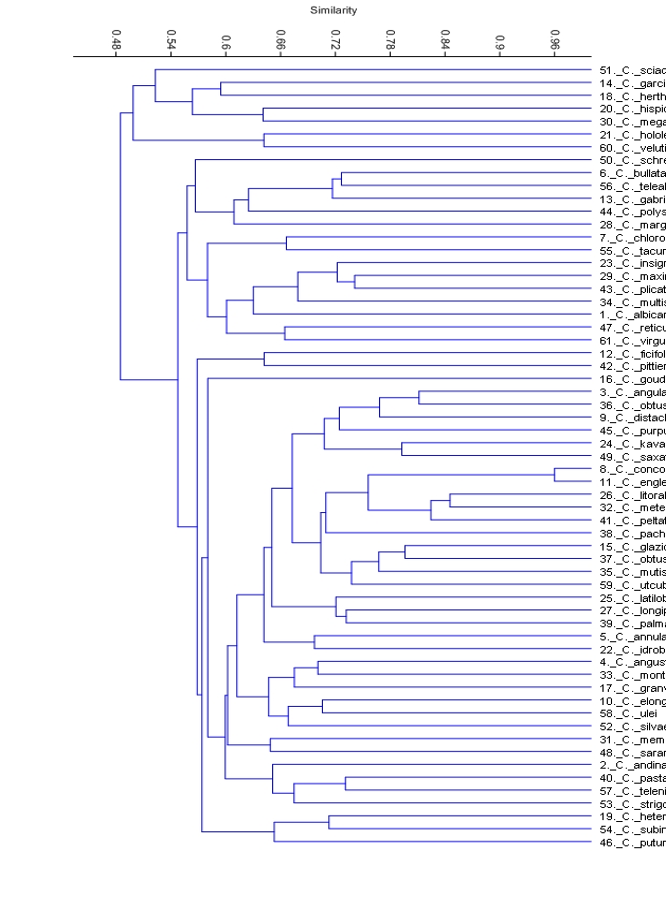
\includegraphics[width=1\linewidth]{figure/fig10a} 

}

\caption{: Classification Ascendante Hiérarchique (CAH) selon la
méthode UPGMA (\textbf{U}nweighted \textbf{P}air \textbf{G}roup
\textbf{M}ethod with \textbf{A}rithmetic Mean) incluant les caractères
quantitatifs et qualitatifs.}\label{fig:fig10a}
\end{figure}






\begin{figure}[H]

{\centering 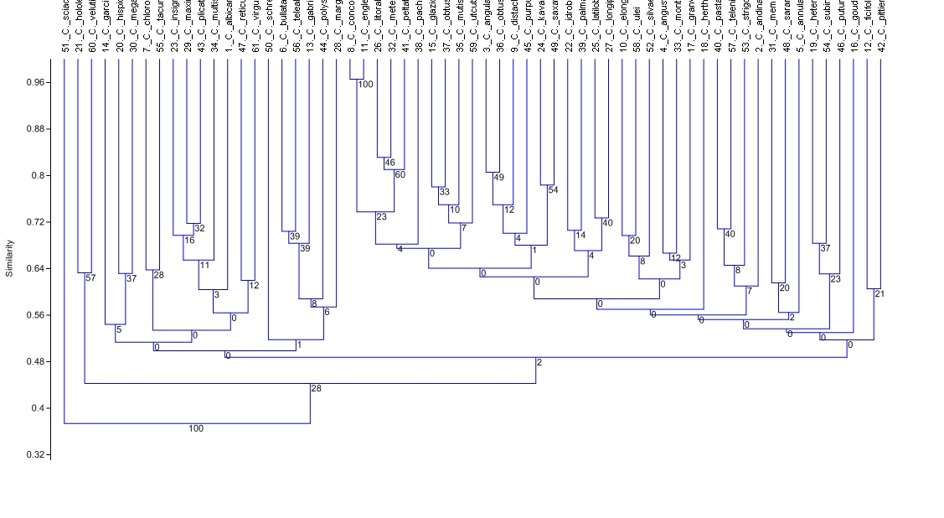
\includegraphics[width=1\linewidth]{figure/fig10b} 

}

\caption{: Classification Ascendante Hiérarchique (CAH) selon la
méthode UPGMA (\textbf{U}nweighted \textbf{P}air \textbf{G}roup
\textbf{M}ethod with \textbf{A}rithmetic Mean) pour les caractères
qualitatifs.}\label{fig:fig10b}
\end{figure}






\begin{figure}[H]

{\centering 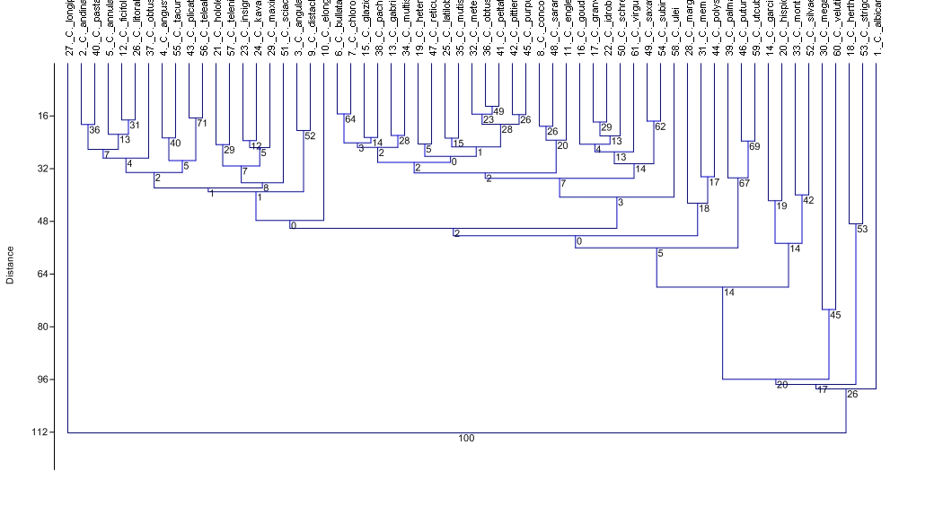
\includegraphics[width=1\linewidth]{figure/fig10c} 

}

\caption{: Classification Ascendante Hiérarchique (CAH) selon la
méthode UPGMA (\textbf{U}nweighted \textbf{P}air \textbf{G}roup
\textbf{M}ethod with \textbf{A}rithmetic Mean) pour les caractères
quantitatifs.}\label{fig:fig10c}
\end{figure}

\subsection{La diversité des espèces Guyanaise : études de
cas.}\label{la-diversite-des-especes-guyanaise-etudes-de-cas.}

Dans la plupart des cas, je n'ai eu aucun mal à identifier les
différentes espèces de Guyane avec ma clef multi-entrée. L'espèce la
plus stable du point de vue des traits morphométriques est sans aucun
doute \emph{C. sciadophylla}. Cependant, plusieurs problèmes ont été
rencontrés et certains morphotypes restent non identifiés.

\textbf{Cas n°1} -- La Figure \ref{fig:fig11} montre un spécimen
photographié par D. Sabatier en novembre 2011 sur la piste forestière de
la Mataroni (N 04°06'13,9" W 52°04'40,1``, Herbier Sabatier D., Smock
J.-L. \& Tarcy M. 5805, CAY). 11 caractères morphométriques sont
observables/mesurables. Alors que l'ensemble de ces critères nous amène
à identifier \emph{C. distachya} sans avoir besoin de renseigner la
localisation géographique, la présence de 6 épis par inflorescence
contredit ce diagnostic. Pour B\&FR2005, le nombre d'épis femelles varie
de 2 à 4. Cette fourchette a été établie à partir de l'observation de 45
échantillons dont deux seulement provenait de la Guyane française. Face
au faible nombre d'échantillon observé par B\&FR2005 et au fait que tous
les critères semblent désigner \emph{C. distachya} en dehors du nombre
d'épis femelles, nous concluons que l'identification est exacte mais que
la variabilité de ce critère est sous-estimé dans l'ouvrage de
B\&FR2005. Nous avons été confronté au même genre de cas (1 ou 2
caractères non conformes aux fourchettes établies par B\&FR2005) pour un
échantillon mâle de \emph{C. distachya} (avec un nombre d'épis trop peu
élevé et des pétioles trop longs), un échantillon stérile de \emph{C.
silvae} (avec des lobes légèrement soudés à leur base) et un échantillon
de \emph{C. obtusa} (avec des nervures tertiaires).

\textbf{Cas n°2} -- La Figure \ref{fig:fig12} montre un spécimen stérile
photographié par P. Heuret en mars 2011 sur la piste forestière de
Counami (N5°21'33'`W53°12'49'', Herbier Heuret n° 123, CAY). 10
caractères morphométriques sont observables/mesurables. Cette
description n'amène à aucune espèce parmi les 61 décrites. Plusieurs
critères entrent à chaque fois en conflit. L'espèce les plus proche de
cette description est \emph{C. angustifolia}. Cependant, celle-ci
possède un indumentum arachnoïde sur le pétiole alors que dans ce cas le
pétiole est glabre. Mais surtout l'échantillon collecté le plus proche
de la Guyane se trouve au Vénezuela à 1700 km. Si l'on regarde les
espèces attendues en Guyane Française, les plus proche sont \emph{C.
sciadophylla} et \emph{C. silvae}. Mais \emph{C. sciadophylla} (i) ne
présente cependant pas de trichilium, (ii) les lobes sont découpés
jusqu'à leur base et s'insèrent directement sur le pétiole et (iii) il
n'y a pas de nervures tertiaires ; ces critères sont ici pourtant
clairement exprimés. Quand à \emph{C. silvae}, les différences avec cet
échantillon sont nombreuses : (i) il possède un indumentum pubérulent ou
hirsute sur le pétiole, (ii) Le nombre de lobes est plus élevé et va de
15 à 20 alors que nous en observons 11, (iii) Le nombre de nervures
latérales est également plus élevé et va de 40 à 58 alors que nous en
observons 32 paires et (iv) il n'y a pas de nervures tertiaires. Cet
échantillon n'est donc conforme à aucune espèce déjà décrite. Après
prospection à l'endroit où il a été récolté, nous n'avons pas été
capable de retrouver un morphotype similaire.

\textbf{Cas n°3} -- Le spécimen que j'ai photographié en avril 2012 sur
la route entre Saint-Laurent du Maroni et Apatou; N5°14'54.3''
W54°15'48.3'' Herbier Heuret\&Nguyen n° 127, CAY (Fig. \ref{fig:fig13}).
A partir de la clef de B\&FR2005 j'arrive à un choix entre \emph{C.
obtusa} et \emph{C. peltata}. Après avoir renseigné 17 caractères avec
ma clef multi-entrées, ces deux espèces sont écartées car elles sont
incompatibles avec 5 et 3 caractères respectivement. Par contre,
j'arrive à une proposition qui est \emph{C. obtusifolia}. Nous sommes
par contre bien loin de son aire de répartition puisqu'elle se trouve
sur la cordillère des Andes en Equateur et Colombie ainsi Amérique
centrale. Je précise cependant que je n'ai pas observé la forme du
stigmate qui est un caractère important.





\begin{figure}[H]

{\centering 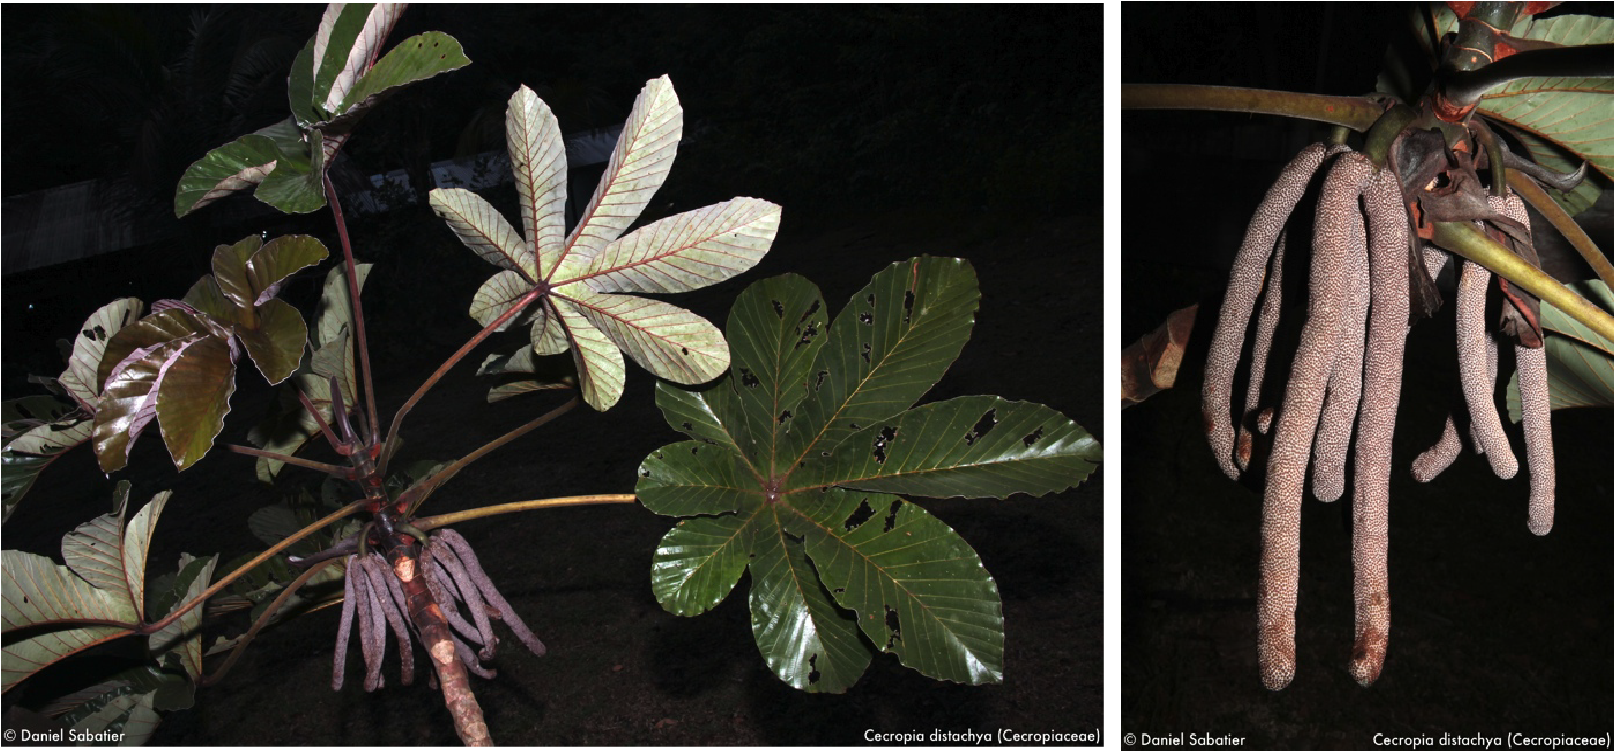
\includegraphics[width=0.8\linewidth]{figure/fig11} 

}

\caption{: Le spécimen photographié par D. Sabatier en novembre 2011
sur la piste forestière de la Mataroni (N 04°06'13,9" W 52°04'40,1``,
Herbier Sabatier D., Smock J.-L. \& Tarcy M. 5805, CAY)}\label{fig:fig11}
\end{figure}





\begin{figure}[H]

{\centering 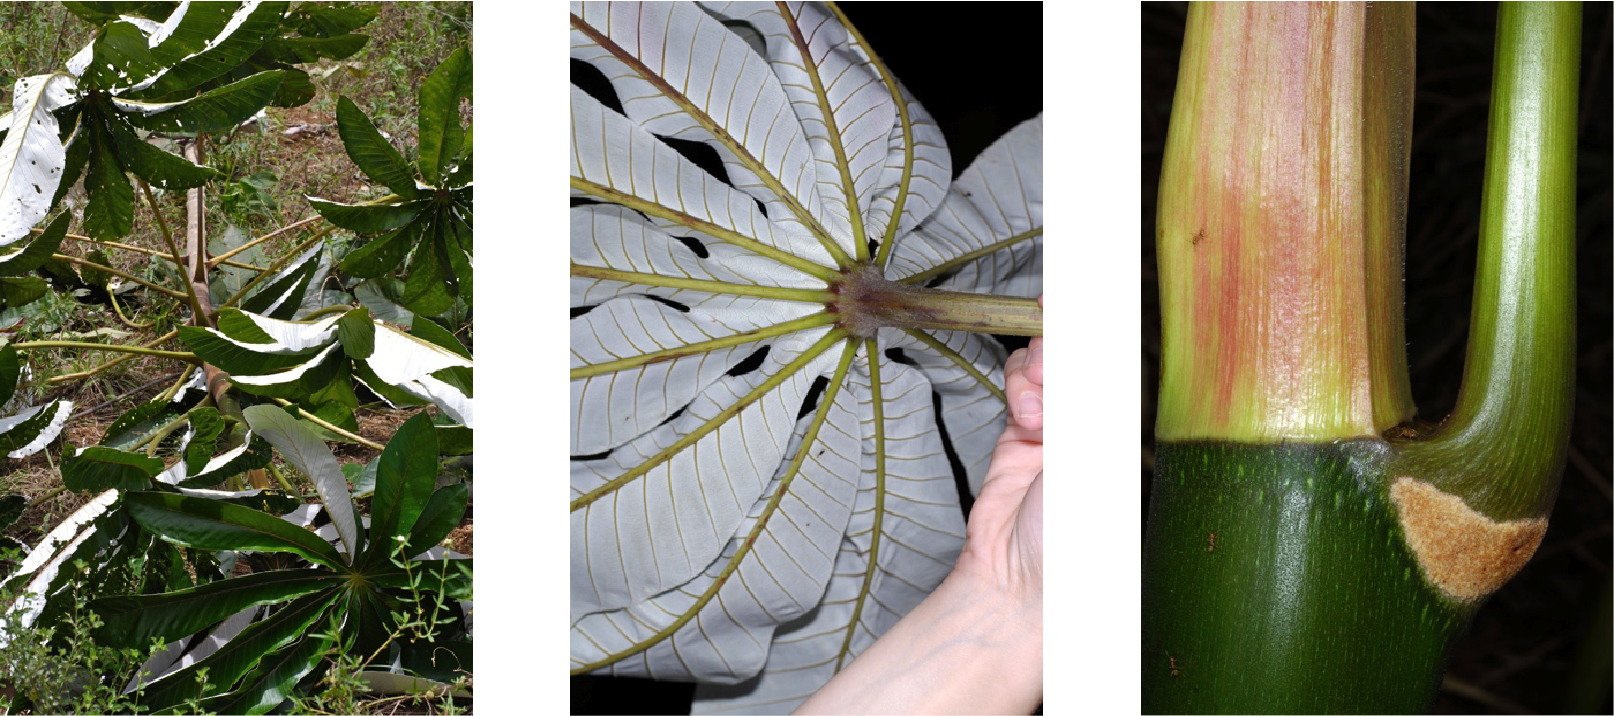
\includegraphics[width=0.8\linewidth]{figure/fig12} 

}

\caption{: Le spécimen stérile photographié par P. Heuret en mars
2011 sur la piste forestière de Counami (N5°21'33'`W53°12'49'', Herbier
Heuret n° 123, CAY)}\label{fig:fig12}
\end{figure}





\begin{figure}[H]

{\centering 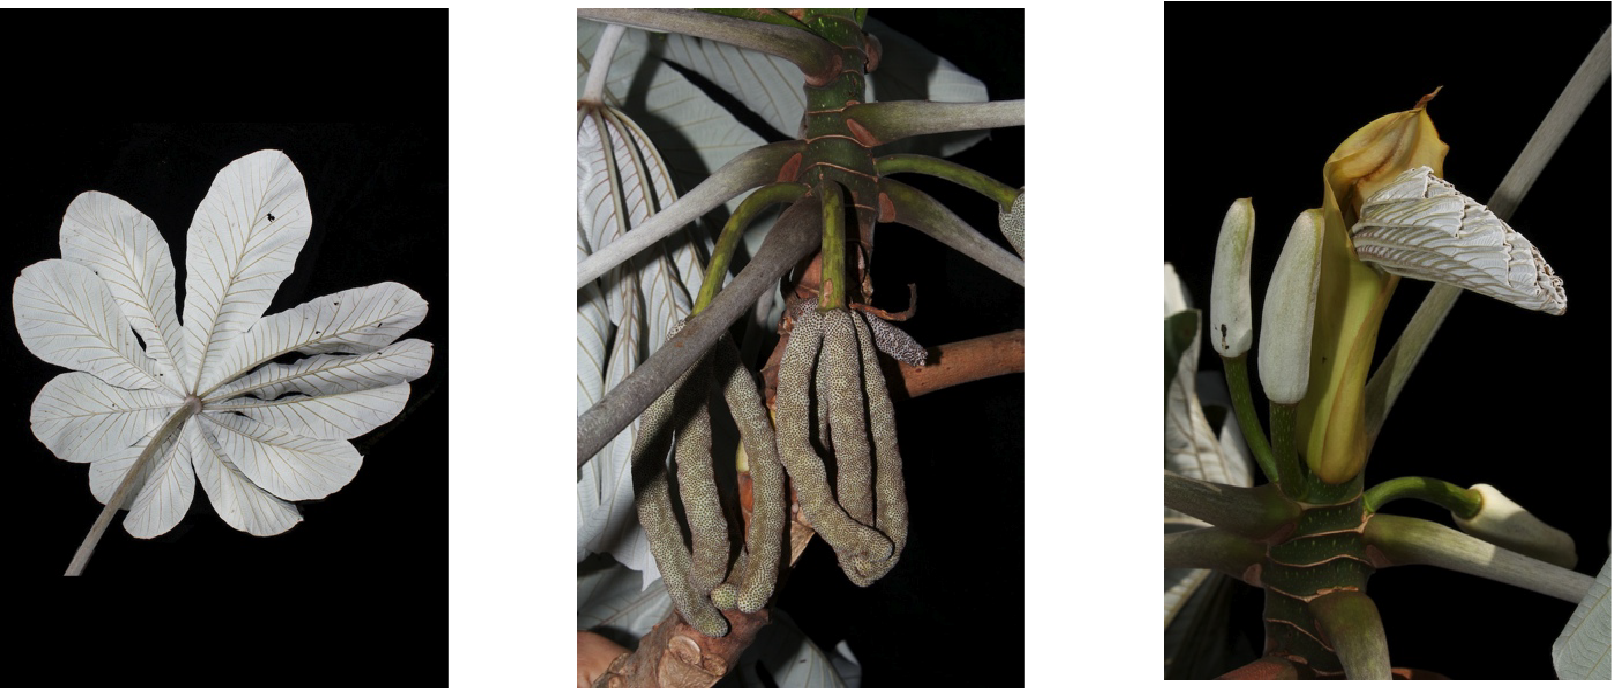
\includegraphics[width=0.8\linewidth]{figure/fig13} 

}

\caption{: Le spécimen que j'ai photographié en avril 2012 sur la
route entre Saint-Laurent du Maroni et Apatou; N5°14'54.3''
W54°15'48.3''; Herbier Heuret\&Nguyen n° 127, CAY.}\label{fig:fig13}
\end{figure}

\pagebreak

\section{Discussion}\label{discussion}

Au cours de ce travail, j'ai réalisé une clef d'identification
multi-entrées en proposant une nouvelle analyse du travail de B\&FR2005.
Sans ce travail remarquable, qui est le résultat d'un nombre
d'observation considérable, rien n'aurait été possible. Cette nouvelle
lecture de cet ouvrage met en avant des critères non considérés par les
auteurs et pourtant pertinents car discriminants. Le développement d'une
clef sous Xper2 offre des possibilités d'identification plus souples,
plus rapides et plus didactiques (grâce aux nombreuses illustrations)
que les clefs dichotomiques à entrées régionales proposées par les
auteurs. Cela permet également d'identifier les \emph{Cecropia}
lorsqu'ils sont exotiques.

Néanmoins les observations que nous avons faites en Guyane montrent que
l'outil ne fait tout. Notre état de connaissance sur les \emph{Cecropia}
reste faible comme le soulignent B\&FR2005 dans leur introduction. Pour
mémoire, 22.54\% des états restent non décrits dans la matrice de
caractère que j'ai synthétisée. Ensuite, nous avons vu que la
variabilité phénotypique des espèces est parfois sous-évaluée en raison
du nombre limité d'échantillon sur lequel pouvaient s'appuyer B\&FR2005
dans les herbiers internationaux. Mais surtout, certains morphotypes ne
trouvent pas toujours de correspondance dans les 61 espèces décrites.
Pour certains spécimens de Guyane, où nous avons pu attribuer une
identification, alors nous nous sommes parfois confronté à une
incohérence géographique, l'espèce attribuée ayant une aire de
répartition très éloignée.

Les causes de ces problèmes peuvent être multiples. Premièrement, il est
fort probable qu'il reste des espèces de \emph{Cecropia} à découvrir.
Ensuite, comme le souligne \citet{Webber2011}, il est probable qu'il y
ait des phénomènes d'hybridations qui rajoutent localement de la
variabilité. L'individu observé sur la piste de Counami (Fig.
\ref{fig:fig12}) pourrait en être un exemple dans le sens que nous
n'avons pas été capable de retrouver un morphotype similaire là ou il
avait été échantillonné. Enfin, il ne faut pas perdre de vue que la
circonscription des espèces proposée par B\&FR2005 puisse dans certain
cas être erronée. Une approche moléculaire fait aujourd'hui cruellement
défaut. Cependant, une telle approche ne pourra venir qu'en complément
d'une étude taxonomique sérieuse et pour cela, nous avons besoin de
nouvelles observations l'échelle de l'aire de répartition du genre.

Les \emph{Cecropia} sont très peu récoltés pour être envoyé dans les
herbiers internationaux. Pour beaucoup de prospecteurs, ce sont des
banalités. Là où plusieurs espèces sont présentes, ils n'en voit souvent
qu'une seule \citep{Berg2005}. Les fourmis agressives qui les habitent,
la grande dimension des feuilles difficile à mettre en presse, la
dioécie sont autant d'obstacles qui freinent leur récolte. Dans ce
travail, j'ai montré que la grande majorité des caractères nécessaires à
discriminer les espèces, sont observables sur un jeu d'une dizaine de
photographies représentant des vues judicieusement choisies. Il est
toujours plus délicat de demander à un collègue de mettre en presse et
d'envoyer un échantillon d'herbier plutôt que de lui demander quelques
photographies qu'il est possible transférer rapidement via internet. Je
pense qu'un `appel à photographie' auprès d'une large communauté
pourrait trouver un écho positif et nous permettre de collecter
rapidement de nouvelles données. C'est en quelque sorte ce que nous
avons fait en demandant à plusieurs collègues leur photographies pour
créer notre photothèque et les réponse furent toujours positives. Il
suffit juste de stimuler de nouvelles prises de vue suivant un protocole
un peu plus cadré. On peut voir cela comme des sciences citoyennes ou en
complément de la communauté scientifique, des amateurs volontaires, des
amateurs éclairés, des spécialistes à la retraite, etc. sont mis à
contribution. Plusieurs niveaux pourraient être envisagés depuis la
simple prise de photographique jusqu'à la récolte d'un herbier et une
descrtiption détaillée des caractères sur la fiche que je propose en
annexe 3 et annexe 4. Au travers d'une vitrine que pourrait être un site
internet dédié à la tribu, nous pourrions ainsi récolter de quoi
construire une matrice de caractère à l'échelle des spécimens et
retravailler la circonscription des espèces et les source de leur
variabilité phénotypique. Il serait particulièrement intéressant de
travailler plus sérieusement la question de la variation des caractères
au cours de l'ontogénie. Par ailleurs, les diamètres de pétiole, de
pédoncule d'inflorescences ou d'épis varient beaucoup de l'état frai à
l'état déshydraté si bien que les valeurs renseignées par B\&FR2005
peuvent induire des biais lors de l'identification de matériel frais. La
récolte de données en frai et en sec et la recherche de règles de
conversion serait également à travailler. La cerise sur le gâteau serait
évidemment d'associer pour chaque spécimen un échantillon ADN permettant
de comparer variabilité morphométrique et moléculaire. \pagebreak

\section{Conclusion}\label{conclusion}

Les outils d'aide à l'identification connaissent un grand succès depuis
une dizaine d'années car ils permettent de rendre la tache bien plus
facile qu'avec des clefs dichotomiques. Ce travail sur le genre
\emph{Cecropia} n'est qu'une illustration supplémentaire de la
performance de ces outils. Une prochaine étape pourrait être de
travailler sur la plate-forme IDAO qui s'affranchit complètement des
définitions botaniques pour raisonner principalement par l'image, au
travers de « portraits-robots ». Quoi qu'il en soit, ces outils doivent
à présent se nourrir de données de terrain pour gagner en précision et
en efficacité. Nous l'avons vu, notre méconnaissance du genre rend
l'identification de certains spécimens difficile. En Guyane française,
qui comporte relativement peu d'espèces par rapport à des pays comme la
Colombie, les choses ne sont pas si claires que cela. En dehors de
\emph{C. obtusa, C. sciadophylla} et \emph{C. palmata} les autres
espèces ont été très peu échantillonnées et sur la nouvelle route
st-Laurent-Apatou plusieurs morphotypes ne sont pas identifiés. Ce
travail donne de premières pistes pour travailler en réseau et compléter
la matrice de caractères. \pagebreak
%\addcontentsline{toc}{section}{References}
\bibliography{book.bib,packages.bib}


\end{document}
